%%%%%%%%%%%%%%%%%%%%%%%%%%%%%%%%%%%
%%%%       Preamble
%%%%%%%%%%%%%%%%%%%%%%%%%%%%%%%%%%%

\documentclass[12pt,oneside]{fithesis2}
\usepackage[backend=biber,style=numeric]{biblatex}
\addbibresource{paperbib.bib}
\usepackage[english]{babel} % package for multilingual support
\usepackage[cp1250]{inputenc} % Windows OS encoding
\usepackage[T1]{fontenc}
\usepackage{quotchap}
\usepackage{graphicx}
\usepackage{rotating}
\usepackage[table]{xcolor}
\graphicspath{{images/}}
\usepackage{csquotes}
\usepackage{pgfplots}
\usepackage{tikz}
\usepackage{subfiles}
\usepackage[section]{placeins}
\usepackage{imakeidx}
\usepackage{tabularx}
\usetikzlibrary{backgrounds}
\usepackage[plainpages=false,pdfpagelabels,unicode]{hyperref}
\thesistitle{Developing a multi-tenant, media-marketplace architecture with Windows Azure and ASP.NET} % enter thesis title
\thesissubtitle{Masters thesis}
\thesisstudent{Aubrey D. Oosthuizen} % name of the author
\thesiswoman{false} % defines author’s gender
\thesisfaculty{fi}
\thesisyear{Winter 2014}
\thesisadvisor{Bruno Rossi, Ph.D.} % fill in advisor’s name
\thesislang{en} % thesis is in English
\makeatletter

\tikzset{%
  fancy quotes/.style={
    text width=\fq@width pt,
    align=justify,
    inner sep=1em,
    anchor=north west,
    minimum width=\textwidth,
  },
  fancy quotes width/.initial={.8\textwidth},
  fancy quotes marks/.style={
    scale=8,
    text=white,
    inner sep=0pt,
  },
  fancy quotes opening/.style={
    fancy quotes marks,
  },
  fancy quotes closing/.style={
    fancy quotes marks,
  },
  fancy quotes background/.style={
    show background rectangle,
    inner frame xsep=0pt,
    background rectangle/.style={
      fill=gray!25,
      rounded corners,
    },
  }
}

\newenvironment{fancyquotes}[1][]
{%
\noindent
\tikzpicture[fancy quotes background]
\node[fancy quotes opening,anchor=north west] (fq@ul) at (0,0) {``};
\tikz@scan@one@point\pgfutil@firstofone(fq@ul.east)
\pgfmathsetmacro{\fq@width}{\textwidth - 2*\pgf@x}
\node[fancy quotes,#1] (fq@txt) at (fq@ul.north west) \bgroup
}
{
\egroup;
\node[overlay,fancy quotes closing,anchor=east] at (fq@txt.south east) {''};
\endtikzpicture
}


\makeatother


\makeindex


%%%%%%%%%%%%%%%%%%%%%%%%%%%%%%%%%%%
%%%%       Document
%%%%%%%%%%%%%%%%%%%%%%%%%%%%%%%%%%%
\begin{document}
\FrontMatter
\ThesisTitlePage
\begin{ThesisDeclaration}
\DeclarationText
\AdvisorName
\end{ThesisDeclaration}
\begin{ThesisThanks}
I would like to thank Dr. Bruno Rossi for acting as my thesis adviser and continuously giving valuable feedback and criticism that guided the thesis into a presentable piece of work. Furthermore I would like to thank Mr. D. Harrison for being my mentor during my internship at XV and providing me with copious amounts of guidance. Finally I would like to thank M. Oosthuizen for being a truly supporting partner through even the toughest of times and keeping me working.
\end{ThesisThanks}
\begin{ThesisAbstract}
Abstract comes here (write at end of thesis)
\end{ThesisAbstract}
\begin{ThesisKeyWords}
Multi-tenancy, Cloud Computing, Software as a Service, SaaS, Cloud Native Application, SaaS Maturity, Architecture Description, Microsoft Azure, ASP.NET, MVC, Command Query Responsibility Segregation, Queue Centric Workflow Computing
\end{ThesisKeyWords}
\MainMatter
\tableofcontents % prints table of contents
%\chapter{Introduction}
The advent of cloud computing \index{Cloud Computing} has changed the way we look at Service Science (SS). With the rapidly declining cost of Infrastructure, Platform and Software as a Service offerings and the increased potential of cloud technologies many are moving away from a classic self-hosting Infrastructure to a cloud alternative. One of the biggest advantages that cloud computing provides is potentially limitless vertical scalability. As a result, software engineers and computer architects have needed to change the way they design and implement their software and systems. This meant stepping back from a single instance, single-tenant model and considering utilizing the advantages the cloud has provided by means of multi-tenancy.\index{Multi-tenant}
 
This study focuses on understanding what multi-tenancy is and why it is relevant to the design of cloud based solutions. A case study is used to provide a relevant context to research from which design considerations are drawn and finally a theoretical architecture implementing multi-tenancy for the specific case requirements is derived.


\section{An Analogy for Multi-tenancy}

A common analogy for multi-tenancy can be made by comparing multi-tenant software systems with an apartment block. Software tenants are considered a closed group of customers that are handled together and usually share a common view of the system \cite{Krebs2012} \cite{Wilder2012-so}. This means that like in the apartment block, tenants are a grouping of customers (people/families/businesses) using the system (living in an apartment). In such an apartment block, a tenant is an owner of their own respective apartment. Each tenant lives and operates within their apartment independently of other tenants. The tenant could also have other people living or working in his apartment while being completely isolated from the apartment block and other tenants as a whole. Although each tenant lives and acts as if they own the entirety of their apartment block, they are actually sharing resources with all the other tenants including electricity, heating and property space. In contrast classical software systems represent a house, where only a single-tenant lives and all resources are consumed and used by that tenant. Building a house for each family (grouping of customers or tenant) is extremely expensive and in many cases simply not feasible. This is especially true since everyone wants to pay the minimum amount of money for a place to live.
 
 \section{Problem}
 
Similar to an apartment, customers and businesses want to keep costs for hosting or using software to a minimum. With applications that are designed and modified for a specific client or tenant and then hosted as an individual instance for that tenant, hosting costs increase linearly per tenant. In addition, all changes required by the tenant are implemented for that tenant's application instance, stacking up development and maintenance costs. If the same application needs to be modified for another tenant, the core application is modified and another instance of the modified application is hosted. This allows for the same application core to be hosted in many instances, each serving a specific tenant. 

Although this model allows for some particular benefits, it does not fit in the current "massive scalability" and "service" based cloud paradigm. Provisioning of new tenants is a manual process and scalability is mostly vertical (higher performance of computer hosting the instance) compared to cloud specialized horizontal scaling (more instances sharing application workload). Furthermore, vertical scaling is usually unidirectional, providing no elasticity. 

Modifications or implementation of new features also need to be implemented for each individual tenant's code base in cases where a separate code base is used. In cases where a single code base is used, switches and checks are overused in order to determine the application behaviour. This dramatically adds to application complexity and reduces maintainability.

\section{Background of the Problem}
The gap between classical hosted and cloud paradigms has given the need for developing multi-tenant solutions. These multi-tenant solutions implement a single application instance in order to serve multiple application tenants while allowing each tenant to extend, configure or modify the application as if they were the sole tenant. Such a multi-tenant system usually comes at a cost of higher design and implementation complexity. However, this increased complexity is usually trivial in comparison to the long term benefits such as the application scalability, availability \index{Availability} and maintainability. Add to this the financial benefits gained by economies of scales, pay per usage models and the reduced cost of commodity hardware, multi-tenant solutions are a powerful alternative for companies looking to gain differential benefit. This is the reason the study introduces exactly such a company as case study. The utilization of a specific case study with its surrounding contexts allows us to obtain a set of design inputs that will be used for defining the architectural constraints and requirements. 

The most important of these being the limitation for our investigation to using Microsoft Azure as our cloud application as well as other Microsoft related products and services. Although research and discussions on multi-tenancy are still limited, three major works of literature are used as the foundation for this study. Firstly, is Microsoft's guide on building multi-tenant application for the cloud using Microsoft Azure \cite{Betts2012-ad}. The guide provides strong theoretical discussions and considerations to take during application design. Although this literature helps one to understand the exact considerations to take when designing the architecture, many of the technologies suggested and used within the guide are now obsolete or have been replaced by better alternatives. This is one of the major influences for this work.

Specific design patterns for the cloud are also fundamental to the construction of such a multi-tenant architecture and are thoroughly discussed \cite{Wilder2012-so}. Finally, methods for addressing the exact specific challenges as set out by our case study is measured through application of Prescriptive Architecture Guidance for Cloud Applications \cite{Homer2014}. 

\section{Statement of the Problem}
In relation to the discussed problem, this thesis aims to answer three questions relating to multi-tenancy with varying degrees of specificity:
\begin{itemize}
\item Which cloud application patterns can be used for the implementation of a multi-tenant application on a variety of cloud platforms?
\item What are the currently available technologies or services provided by Microsoft Azure to create, architect and implement a multi-tenant solution that fits our case study?
\item Which Azure specific multi-tenant architecture can be implemented as prototype \index{Prototype} artefact to solve the major requirements for our case study?
\end{itemize}

\section{Thesis Statement}
This study focuses on multi-tenant application design using Microsoft Azure as cloud platform in order to determine a solid application architecture that would resolve the major requirements of the case study. All this is done in order to better understand the role, design and implementation of multi-tenant applications for the cloud. From this, the following thesis statement has been made:
 
\begin{fancyquotes}
This thesis aims to create a software architecture as artefact that is scalable, customizable and multi-tenant efficient. The artefact should also address the issues and concerns outlined by the case study and be designed around its specific requirements
\end{fancyquotes}

\section{Purpose and Methodology of the Study}
\index{Methodology}

This study relies on design science as it is primarily a problem solving paradigm \cite{Hevner2004}. It is characterized by the creation of a research artefact in the form of models, methods or instantiations that enable researchers to understand the problems related to the development and implementation of Information Technology (IT) and information systems \cite{March1995a}. These artefacts are created by the extension of existing kernel theories that are then applied, tested and modified through the experience, creativity and intuition of the researcher \cite{Walls1992}. In many cases design science is applied in order to solve identified organizational problems. In such cases, the resulting artefact allows researchers to understand the efficiency and feasibility of the artefact as solution to such a problem \cite{Hevner2004}.
 
In this study we use qualitative means to assess and evaluate means of design, implementation and improvement of the artefact. This evaluation provides feedback and allows one to understand the problem better in order to improve the artefact and its design process continuously. It is common for the design artefact to continuously evolve as research is conducted and new theories or directions are undertaken \cite{Hevner2004}.
 
The artefact which is the primary aim of the research is a design model. Hevner et. al \cite{Hevner2004} defined models as a set of connections between problem and solution components that enable exploration of the effects of design decisions and changes in the real world. Therefore, the creation of a "multi-tenant architectural model" can be seen as the principal goal of the research. The secondary supporting artefact is created as means to show the feasibility, allow assessment of, and prove the validity of the primary artefact. This artefact is an instantiation typed artefact \cite{Hevner2004} in the form of a prototype. The prototype aims to implement the minimal features outlined by the primary artefact in order as merely supporting element. The completeness of effectiveness of the design artefact is evaluated in relation to its completeness in addressing the requirements of the original problem as well as its validity to the use case context \cite{Hevner2004}. It is important to keep in mind that since design science is an iterative approach starting with a simplified conceptual presentation of the problem which is assessed in a changing technological and organizational environment that research assumptions are subject to change \cite{Johansson2000}.


\section{Relevance of the Topic and Research}

As most research revolving cloud technologies are still relatively new and continuously changing, it is hard to establish true relevance of a research topic for an extended period. In order to contribute to the pool of knowledge, research should provide results that could be perpetually used in order to improve the deep knowledge in current trends at an appropriate speed to their development. Therefore this research claims relevance in the current interest in cloud technologies and their ability to allow multi-tenant systems to be used as "cloud ready" alternative architecture. Thus, the artefact produced as research results should address the observational requirements of the case study providing a relevant model considering current technologies which could be used either by organizations wishing to implement a multi-tenant system with a similar context or other researchers that wish to extend the model for other technologies, use cases or problem domains. Finally, scientific research should be evaluated in light of its actual practical implementations, proving its relevance to the field and as research \cite{Hevner2004}. This paper aims to evaluate its practicality through observation and application to the research case study.


\section{Research Objectives}

The research problem is approached by firstly evaluating current and related cloud literature. Context to the research problem is then provided through means of the XV Application (XVA) use case. This use case is used as primary design input from which requirements, constraints and considerations are taken where after an in depth dissection of available technologies provided by Microsoft Azure is done. A broad overview of relevant design patterns is given and taken into account before creation of the initial architectural artefact or model. The model is then used to extract a general model for implementation of an multi-tenant application and the Azure specific model is then used to implement an simplistic prototype which is used as "proof of concept" and validity for the architectural model.





\section{Research Outline}

Chapter 1 introduces the problem domain of this thesis and aims to familiarize the reader with the background to the problem and its relevance for investigation. It also clearly explains the intent of the research. The next chapter introduces us to multi-tenancy and its implementation in the cloud. It also examines different levels of Software as a Service (SaaS)\index{Software as a Service (SaaS)} maturity in order to provide grounds for the necessity for SaaS providers to consider multi-tenancy as a crucial part of their software design architecture.
%\chapter{Multi-tenancy}
\index{Multi-tenant}
This chapter aims to introduce the concepts and ideas surrounding multi-tenancy and explain why it is relevant or even important to current cloud computing \index{Cloud Computing} practices.

\section{The Cloud}

Cloud computing is commonly defined as a form of computing where computing resources are shared in contrast to having local dedicated resources to run applications or services \cite{webopedia}. Walker \cite{GraceWalker} further defines cloud computing as a solution that delivers IT as a service by using computers to work together and applications to utilize these collective computing power as a single system.
 
The creation of public clouds, which offer cloud solutions to the general public, has provided anyone with almost unlimited resources and scalability. Large numbers of companies are shifting to using public clouds instead of maintaining their own data centres. The large cost advantages resulting from using the public cloud is the primary factor fuelling this shift, allowing stronger competition between companies of all sizes. Although cloud computing is not a new technology, but simply a way that computing resources are delivered (much akin to historic mainframes). It is a major paradigm shift in the way information and services are provided \cite{GraceWalker}. All of this has created a need for radical redefinition of our current computer architectures, software, tools, persistence mechanism and design patterns \cite{GraceWalker}. Applications design should be continuously aware of the cloud computing layers including Infrastructure as a Service (IaaS), \index{Infrastructure as a Service (IaaS)} Platform as a Service (PaaS)\index{Platform as a Service (PaaS)} and Software as a Service (SaaS), \index{Software as a Service (SaaS)} and be designed to natively support deployment and management through them. Bill Wilder \cite{webopedia} defines applications as cloud-native \index{Cloud-native} if they are architected to take advantage of proven engineering practices that utilize cloud platform services to cost efficiently and automatically allocate resources allowing horizontal scaling, handle hardware failures without downtime and minimize network latency, all automatically.


\section{What is Multi-tenancy?}

Krebs defines multi-tenancy as an approach to share a single application instance between multiple tenants by providing each tenant a dedicated share of the instance which is isolated from other shares with regards to performance and data privacy \cite{Krebs2012}.
Wilder \cite{Wilder2012-so} defines multi-tenancy as a system shared by tenants, usually operated by a single company. Furthermore, Bezemer goes on to extend these definitions by stating that multi-tenant applications should allow tenants to configure the application to meet their specific needs as if it was running on a completely dedicated environment\cite{Bezemer:2010:MSA:1862372.1862393}. While these definitions do thoroughly express the basic principle of multi-tenancy, in a broader sense, it does not provide a strong view from which such systems can be architected. It is therefore that I attempt to provide a more concise, amalgamated and personal definition of multi-tenancy in respect to this research as follow:
\\
\begin{fancyquotes}
Multi-tenancy is a [software] architecture principle which dictates the sharing of physical computing resources by groupings of tenants by utilizing a single application instance that is limitlessly, horizontally scalable, while logically isolating each one of its tenants.
\end{fancyquotes}
\\
This definition, however leaves to question the exact meaning of a tenant. One definition of a tenant is a grouping of customers that are a closed, charged and handled together \cite{Krebs2012}. Bezemer suggests that these groupings are stakeholders in an organization  \cite{Bezemer:2010:MSA:1862372.1862393} while Wilder defines tenants as specific groupings of users that have their own respective employees or customers that can access the system while sharing a common view \cite{Wilder2012-so}.
Some of the key aspects of multi-tenant applications has been summarized as follow \cite{Bezemer:2010:MSA:1862372.1862393}
\begin{enumerate}
\item The application should be able to share hardware resources
\item The application should be highly configurable
\item  The application should use a single instance and in pure multi-tenant solutions, even a single database instance should be used
\end{enumerate}

\section{An Analogy for Multi-tenancy}

A common analogy for multi-tenancy can be made by comparing multi-tenant software systems with an apartment block. Software tenants are considered a closed group of customers that are handled together and usually share a common view of the system \cite{Krebs2012} \cite{Wilder2012-so}. This means that like in the apartment block, tenants are a grouping of customers (people/families/businesses) using the system (living in an apartment). In such an apartment block, a tenant is an owner of their own respective apartment. Each tenant lives and operates within their apartment independently of other tenants. The tenant could also have other people living or working in his apartment while being completely isolated from the apartment block and other tenants as a whole. Although each tenant lives and acts as if they own the entirety of their apartment block, they are actually sharing resources with all the other tenants including electricity, heating and property space. In contrast classical software systems represent a house, where only a single-tenant lives and all resources are consumed and used by that tenant. Building a house for each family (grouping of customers or tenant) is extremely expensive and in many cases simply not feasible. This is especially true since everyone wants to pay the minimum amount of money for a place to live.

\section{Multi-tenant vs. Single-tenant}

The difference between multi-tenant and single-tenant systems can clearly be outlined as in figure \ref{fig:multi-vs-single}. This diagram shows how an applications logical instance is shared by different clients in a multi-tenant system. Using multiple physical instances of an application is an easy way to scale the application to handle higher loads, especially when combined with a load balancer to serve users of the single specific client's logical instance to the different physical instances. Prime examples of multi-tenancy in this form, is the public cloud providers themselves. Azure, for example, runs its PaaS services on shared hardware. While allowing companies (tenants) to use its PaaS as if they are the exclusive tenants to serve their own respective customers or employees.
Further distinction is required between multi-tenancy, multi-instance \index{Multi-instance} and multi-user. Multi-user applications are simply applications that supports multiple users. In essence, there is no grouping of customers and all customers are treated equally\cite{Bezemer:2010:MSA:1862372.1862393}. In contrast, many multi-instance applications group users together and thus each application instance is configured to serve one tenant. Multi-tenant applications, however, are assumed to be highly configurable at the tenant level providing a dedicated instance feeling while in reality running on a single instance \cite{Bezemer:2010:MSA:1862372.1862393}.

\section{SaaS and Multi-tenancy}

A simple definition for SaaS as defined by Chong \cite{Chong2006} as software deployed as a hosted service and accessed over the internet. Well architected SaaS solutions are usually evaluated by their ability to scale and serve multiple tenants efficiently and allows configuration. Therefore, it is fundamental for any SaaS provider and their software architects to understand the impact and means of achieving multi-tenancy.

\section{Maturity Level}

A common benchmark for measuring the maturity level of a SaaS application is the SaaS Maturity Model (see figure \ref{fig:saas_maturity_model}). This figure indicates the different levels of SaaS maturity. Level 1 is similar to traditional hosted application or application service provider (ASP) model. Each customer of this SaaS provider has its own customized version of the hosted application and each hosted version runs as a singular instance on the provider's servers. Within level 1, all application instances are independent and any customization made to the code needs to be replicated to all applicable instances and redeployed. This level is common for providers that migrate, their in -house hosted applications to the public cloud. The second level of SaaS maturity is the unification of all application instances to a single instance, hosted once for each of the tenants. Additionally, the 2nd level allows customization not by altering the application code, but by allowing for customization through configuration. This model is useful since single-tenant application instances can be scaled vertically and only a single code base needs to be maintained. The third level of maturity introduces multi-tenancy as its core requirement. Having a single instance of the application running and serving multiple tenants. Configuration on the third level is also done through configuration and tenant's data is logically isolated. To the individual tenant, it appears as if they are the sole consumers of the service. This level allows for efficient sharing of computing resources and simplifies management and coding efforts although it inherently has limited vertical scalability due to the singular instance of the application. In enabling the SaaS service to be horizontally scalable, the 4th maturity level can be reached. With the 4th level, identical application instances are hosted and a load balancer distributes the load between these instances. This is the ideal maturity level for any SaaS application as it allows for limitless horizontal scaling with elasticity, effective resource sharing, high availability \index{Availability} and easy maintainability. This model clearly shows the need for any SaaS provider to understand and put into effect multi-tenancy as part of its application architecture in order to build truly effective, cloud-native\index{Cloud-native} SaaS applications.

\section{Why Multi-tenancy?}

Cloud computing offers boundless capacity for scaling out (vertical scaling) and allows us to create new instances of whichever service we require on the fly. Cloud platforms in themselves are optimized for cost-efficiency. In its essence, cloud platforms themselves are multi-tenant systems with multiple tenants sharing IaaS, PaaS or SaaS services while running on commodity hardware \cite{Wilder2012-so}. In order to truly make use of the advantages provided by cloud computing, especially for scaling and fault tolerance. Using a multi-tenant architecture is one of the most efficient methods for SaaS providers to use cloud capabilities to provide high levels of costs saving.
Some of the economical advantage delivered by using multi-tenancy over a single instance model includes \cite{Betts2012-ad}:
\begin{itemize}
\item Reduced costs of maintainability: Provisioning of new tenants are central and require little to no effort and in a mature SaaS model can be done automatically
\item Reduced costs of customization: Customization is done through configuration, therefore removing the need for physically customizing the underlying code
\item Reduced costs of scaling: Since scaling can be done horizontally and elastically, only the amount of application instances needed, for the time they are necessary are used and paid for
\item Reduced costs of hosting: As only a single application instance is hosted to serve multiple tenants, overall hosting costs are reduced. With higher degrees of multi-tenancy, even the database instance is shared by tenants allowing for even further reduction in hosting costs
\item Reduced complexity of implementing new feature development: With the traditional single instance model, any features developed for one tenant needs to be implemented in each one of the other tenants code base, this leads to increased complexity and maintainability. The single multi-tenant instance allows for feature development to be done once and enabled for all tenants
\item Single code base: Since all tenants run the same application instance, only a single code base is maintained for all tenants
\end{itemize}

Although these advantages might make multi-tenancy seem as an obvious choice for cloud application design, there is an extremely important caveat to consider, namely complexity. Figure \ref{fig:imp_complexity} indicates the cost and complexity per tenant between maturity level 1 (single-tenant/ad-hoc) approaches compared to level 4 (scalable, customizable, multi-tenant) implementation. Initial development costs and complexity for multi-tenant solution are higher due the increased expertise, architecting, development and 'time to market' of the application. However, once more tenants are required, the SaaS application costs for level 1 development tends to escalate as each tenant requires their own hosted application instance as well as customization. This trend continues as more tenants are added and quickly the initial costs of implementing a scalable, customizable, multi-tenant-efficient solution becomes the more economical option.


\begin{figure}
\centering
\begin{tikzpicture}
\begin{axis}[
        ymajorticks=false,
    xmajorticks=false,
    xlabel={Tenants},
    ylabel={Cost \& Complexity},
    ymajorgrids=false,
    xmin=-4, xmax=2,
    grid style=dashed,
]
 
\addplot[color=blue]{exp(-x)};
	
	\addplot[color=black] {0.5(x+5)^2 + 20	};
	
\legend{Level 4, Level 1}
\end{axis}
\end{tikzpicture}

\caption{Implementation complexity per tenant}
\label{fig:imp_complexity}
\end{figure}






SaaS maturity level 4 is, however, the archetypal ideal maturity level to execute, but because of its complexity is not always the first multi-tenant level developed by service providers (SP). The 3rd maturity level is also multi-tenant enabled, but does not allow for scaling and therefore inherently contains some risks associated with it such as single point of failure and application instability. Since all tenants share this common instance, the impact of these risks are also (much higher) than with single-tenant applications and should therefore be kept in mind during application design.

\section{Challenges and Requirements of Implementing Multi-tenancy}

Multi-tenancy introduces many common challenges and requirements that need to be addressed in order to be implemented effectively. Common challenges include \cite{Betts2012-ad}:

\begin{itemize}
\item Partitioning
\item Extensibility
\item Provisioning
\item Testability
\item Customization
\item Third Party Components
\item Tenant isolation
\item Security
\end{itemize}

Betts \cite{Betts2012-ad} additionally outlines some of the common requirements a multi-tenant solution should consider and address from the tenant's perspective (see table \ref{table:tenant-requirements}).


These requirements are very important to recognize as they can influence a SP choice of whether or not to design their application to be multi-tenant enabled. For example SP that do not require the scalability and availability, but high levels of security and regulatory compliance might rather implement a single-tenant application that physically isolates its tenant's data.


\section{Conclusion}

This chapter took an overall look at multi-tenancy as an alternative architectural principle used for developing effective SaaS services that utilize many of the advanced capabilities offered by cloud computing. Furthermore, the different levels of SaaS maturity are discussed in relation to multi-tenancy and highlights how fundamental multi-tenancy is to developing good SaaS application. Finally, the economic impact of multi-tenancy is discussed as driving force behind the choice for it to be implemented. The next chapter introduces us to the methodology used in this paper and examines the specifics of how our research problem will be tackled. 

%\chapter{Methodology}

In this chapter an overview of the methodologies, paradigm and process used in order to construct our application architecture is given. It briefly introduces design science as research paradigm and explains how this paper uses design science in order to produce a model as artefact. Furthermore, the use of case study as tool is discussed and justified. Finally, the use of an implementation artefact in the form of a prototype is used in order to evaluate the validity of the model is examined.

\section{Design Science Paradigm}

Henver \cite{Hevner2004} cites the two major paradigms that encapsulate the majority of Information System research as the behavioural and design sciences. Design science is in effect the science of artefacts and is therefore concerned with the design, development, improvement and understanding of artefacts for the purpose of solving problems and implementing IT systems \cite{March1995a}. Artefacts can be in the form of constructs, models, methods or instantiation \cite{Hevner2004}. These artefacts are created by the extension of existing kernel theories that are then applied, tested and modified through the experience, creativity and intuition of the researcher \cite{Walls1992}. Design science is also commonly used to solve identified organizational problems. In such cases, the resulting artefact allows researchers to understand the efficiency and feasibility of the artefact as solution to such a problem \cite{Hevner2004}.
 
March \cite{March1995a} dictates that design sciences does not pose theories but instead aim to create artefacts which are subject to two basic activities, build and evaluate. Therefore it is important to gather adequate information in order to construct an artefact according to specific requirements and then to evaluate this artefact using formal metrics. This paper aims at creating an artefact of the model type. This model should be a detailed architectural description of the interaction between different constructs that make up an effective multi-tenant SaaS application. Significant difficulties in design science are a result of the fact the evaluation such as performance of the artefact is related to the environment within which the artefact it operates \cite{March1995a}.


Combined with the subjectivity of the intended use and users of the actual artefact, makes evaluation a complex task. In order to evaluate the viability of this papers resulting (model) artefact, an (instantiation) artefact in the form of a prototype will be created. The prototype will also provide information on different other aspects of the implementation of the model such as feasibility, complexity and general application stability. Since the prototype artefact is not the target artefact examined by this paper but a means of evaluation, further specific tests to provide empirical data for analysis and evaluation of the prototype has not been included. However, several tests that could theoretically provide useful quantitative data includes stress testing/load testing the service to measure its ability to scale effectively. Additionally using monitoring tools such as Microsoft Application Insights \cite{AppINsight} and acceptance testing.

 
The development of a model artefact shares common traits with classical science in the sense that it attempts to simplify a complex phenomenon in order to be studies. Dodig-Crnkovic \cite{Dodig-crnkovic} suggests that the modeling process attempts to answer six questions relating to the phenomenon:

\begin{enumerate}
\item How should the model be constructed? Which features should be included and which neglected?
\item The appropriateness of the model should be measured in terms of its purpose, resolution and abstractness.
\item The exact features and behaviour of the model should be measured in comparison what is expected.
\item In which ways does the model itself differ from that of reality?
\item Is the model valid?
\item Which external or special constraints should be taken into consideration?
\end{enumerate}

These questions are used as guideline for constructing our model artefact and will be attempted to be answered in order to maintain some degree of relevance to the scientific method. Amaral \cite{Amaral2011} refers to design science as a "build" methodology which creates either a physical artefact or a software system in order to demonstrate that it is indeed possible to be created. Furthermore, Amaral reasons that in order for this methodology to be considered research, the construction of the artefact should not have been created before. Thus the artefact as such should contain new features or processes that have not been demonstrated before. Both the artefacts resulting from this paper attempts to apply features in a combination that has not been done in previous research. This is achieved using technologies that are extremely young (less than a month) old at time of writing and combining these with the specificity of the use case.


\section{Case Study}

In many research papers, a case study is used as the initial foundation by offering a complex research question while providing the proper context within which the problem should be solved \cite{Schell1992-cm}. In order to design an effective architecture or "model artefact", it is important to gather as many necessary design inputs in order to formalize the requirements and constraints that your architectural model should accommodate beforehand \cite{Microsoft_Patterns_Practices_Team2009-ek}. Case studies offer a comprehensive set of functional, non-functional, technological, and infrastructural requirements.
Case offers a much stronger context for implementation by others sharing similar a conditions and is therefore non-classical in the IT sciences. This thesis attempts to similarly create a complete context by providing domain information and system requirements used for creating the model artefact through a case study.


\section{Prototyping}

Prototyping is a powerful demonstration tool. A prototyped artefact aims to act as a pilot case or proof of concept showing that a concept or idea is viable in reality. Furthermore, a prototype aims to provide means for the collection of further specialized data in order to be reused for research purposes. In software engineering, prototyped software should be considered a special kind of software that does not aim to provide actual business value but instead provide grounds for exploration and data gathering \cite{Monperrus2013}. Due to this nature, prototyped software does not need to necessarily comply with common software design practices. Software written as prototype also only aims at working in preset limited amount of use cases and does not need to provide extended support or maintenance \cite{Monperrus2013}. Ideally software prototypes are tools for aligning ideas and attempting to simulate the ability to convert these ideas into reality. It is therefore important to note that the prototype created as part of this paper does not aim to provide specific implementation details or showcase specific design patterns or approaches. It also does not attempt to be a fully fledged system intended for future extension into an actual SaaS service but only exists as means of evaluating the architectural viability.


\section{Qualitative Approach}

A mostly qualitative effort has been used as means to evaluate the model artefacts design. This includes subjective knowledge provided by the implementation of the prototype in order to prove the models viability. This qualitative analysis of findings and experiences is used to further assess and evaluate the efficiency of design, implementation and suggest future improvements. As this paper is also a business oriented project compared to pure research based one, many of the results are based on the subjective view of its intended users and developers. Additionally, the model artefact is evaluated through using the SaaS maturity model as reference point and comparison. This maturity level is then combined with the requirements of the case study in order to determine if the design requirements of the model have been met. Finally the level of maturity reached by the architecture model is assessed and used in order to determine if the study has provided a relevant artefact as result.


\section{Conclusion}

In the next chapter we take a look into our XV Case study and explain the context used as baseline for the rest of the study.


%\chapter{Case Study}

This chapter introduces the XV Application (XVA) as the research case study in order to illustrate the application of multi-tenancy to a real world SaaS application as example. It aims to define a concrete set of design inputs and requirements combined with the current context of the XV SaaS application and attempts to use it as premise for architecting our multi-tenant model.

\begin{figure}
\centering
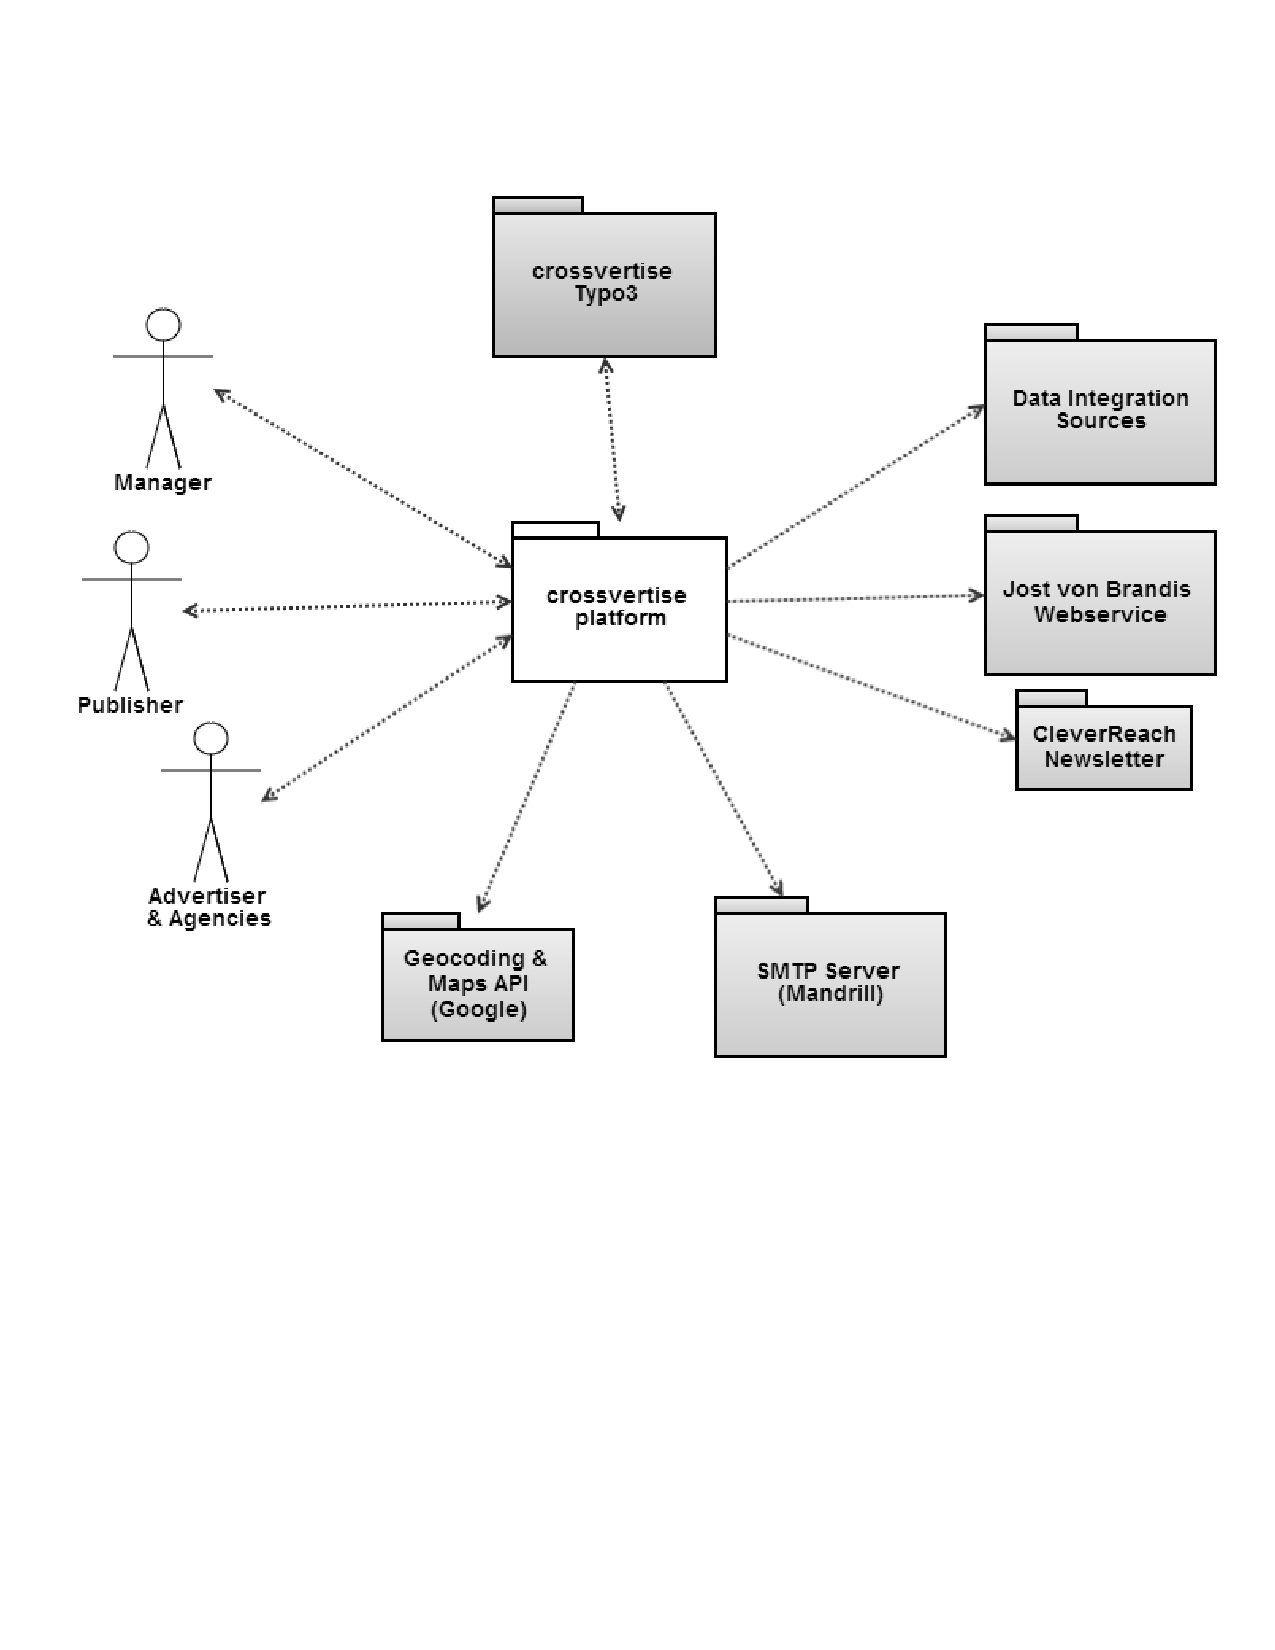
\includegraphics[width=\textwidth]{cross_use_case}
\caption{XV Use Case!!!!!!!!!!!!!!!!!!!!!!!!!!}
\label{fig:cross_use_case}
\end{figure}

\section{XV GmbH}

Crossvertise GmbH henceforth "XV", is a Munich based SaaS provider and start-up. Their core domain of business consists of the entirety of the advertising market. The company has developed their own online, cross-media marketplace application which is offered as SaaS solution to large advertising houses and corporations. Their application is also the back end of their own market.XV.com website which allows publishers, advertisers and companies to run cross-media marketing campaigns by booking advertising media online.
 
The XV Application (XVA) integrates over 80\% of Germany's advertising and publishing data to enable its users to book mobile, online, cinema, television, radio or out-of-home advertising easily and effortlessly online.

\begin{figure}
\centering
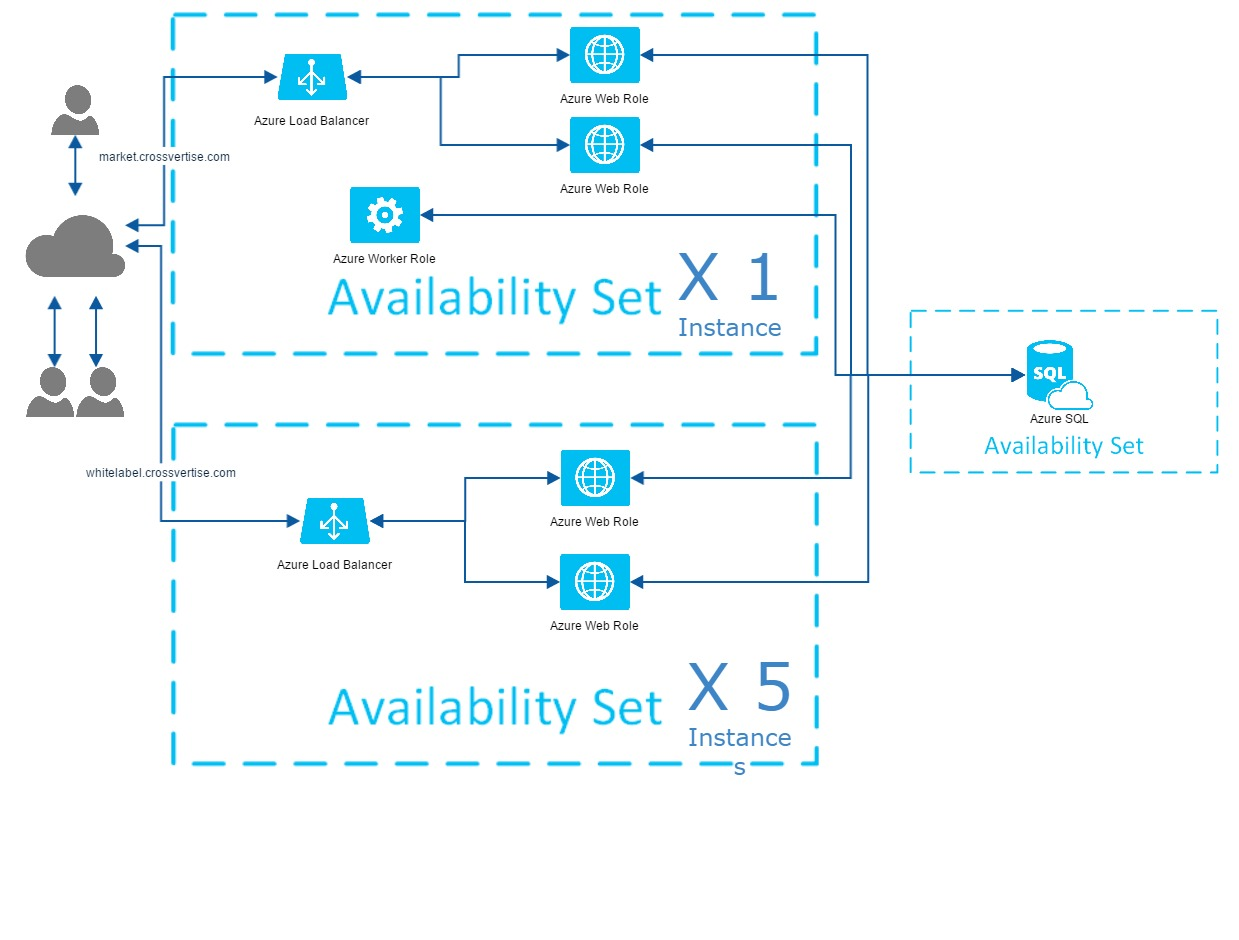
\includegraphics[width=\textwidth]{xv_azure_arc}
\caption{XV Conceptual Architecture Blueprint}
\label{fig:xv_azure_arc}
\end{figure}

\section{The XVA Background}

The current XVA was initially developed as back end to run the companies own media marketplace e-commerce website. However, as time passed it became apparent that they could be a powerful service to be delivered through the public cloud as a SaaS solution for companies that are in the same business domain. Due to this duality in function the application currently only reached SaaS maturity level 1 (ad-hoc) \cite{Chong2006} in the sense that a single, completely customized instance of the application is hosted for each of the application tenants. Since tenants are large advertising companies and have very specific requirements pertaining to the media and mediums which should be provided by their application instance, it has been hard to be able to migrate the service to a higher maturity level. Recently however an active effort has been made by the development team to migrate customization away from code and into configuration in order to achieve SaaS maturity level 2.
 
 
 
At time of writing XV was running 12 instances of their XV Application on Windows Azure Web Roles. Two instances to serve their main website (market.XV.com) and ten instances each serving their individual tenants. Running 12 instances of the same application however is quite costly and has led to the requirement of looking into developing a feasible alternative. The high amount of hosted application instances also contributed to maintenance and administration overhead which could be simplified by a multi-tenant alternative. Finally, the current application persistence model lacks tenant isolation and therefore is a strong candidate for improvement. All of these factors have led to the requirement of moving the current application to a completely scalable, multi-tenant-efficient SaaS solution that meets the criteria of maturity level 4, reduces costs and simplifies tenant provisioning, customization and maintenance.




\subsection{Technical Analysis of the XVA}
\label{sec:techconst}
As a start-up company, XV has subscribed to Microsoft's BizSpark program which helps start-ups engage in software development by providing them with open access to many of Microsoft's technologies and tools \cite{BizSpark}. This has allowed the company to gain access to the public cloud through Microsoft Azure and develop its application using Visual Studio, C\# and ASP.NET Model, View Controller (MVC). Access to these resources have been the primary decisive factor in choices of technologies used in the application and the current IT team has been structured largely around these Microsoft technologies. It is for these reasons that this research paper has continued to use technologies and tools that align with this strategy, however in cases where newer technologies have become available they have been taken into consideration.
 
 
A more precise breakdown of application technologies can be seen in \ref{fig:tech_breakdown}.

\begin{figure}
\centering
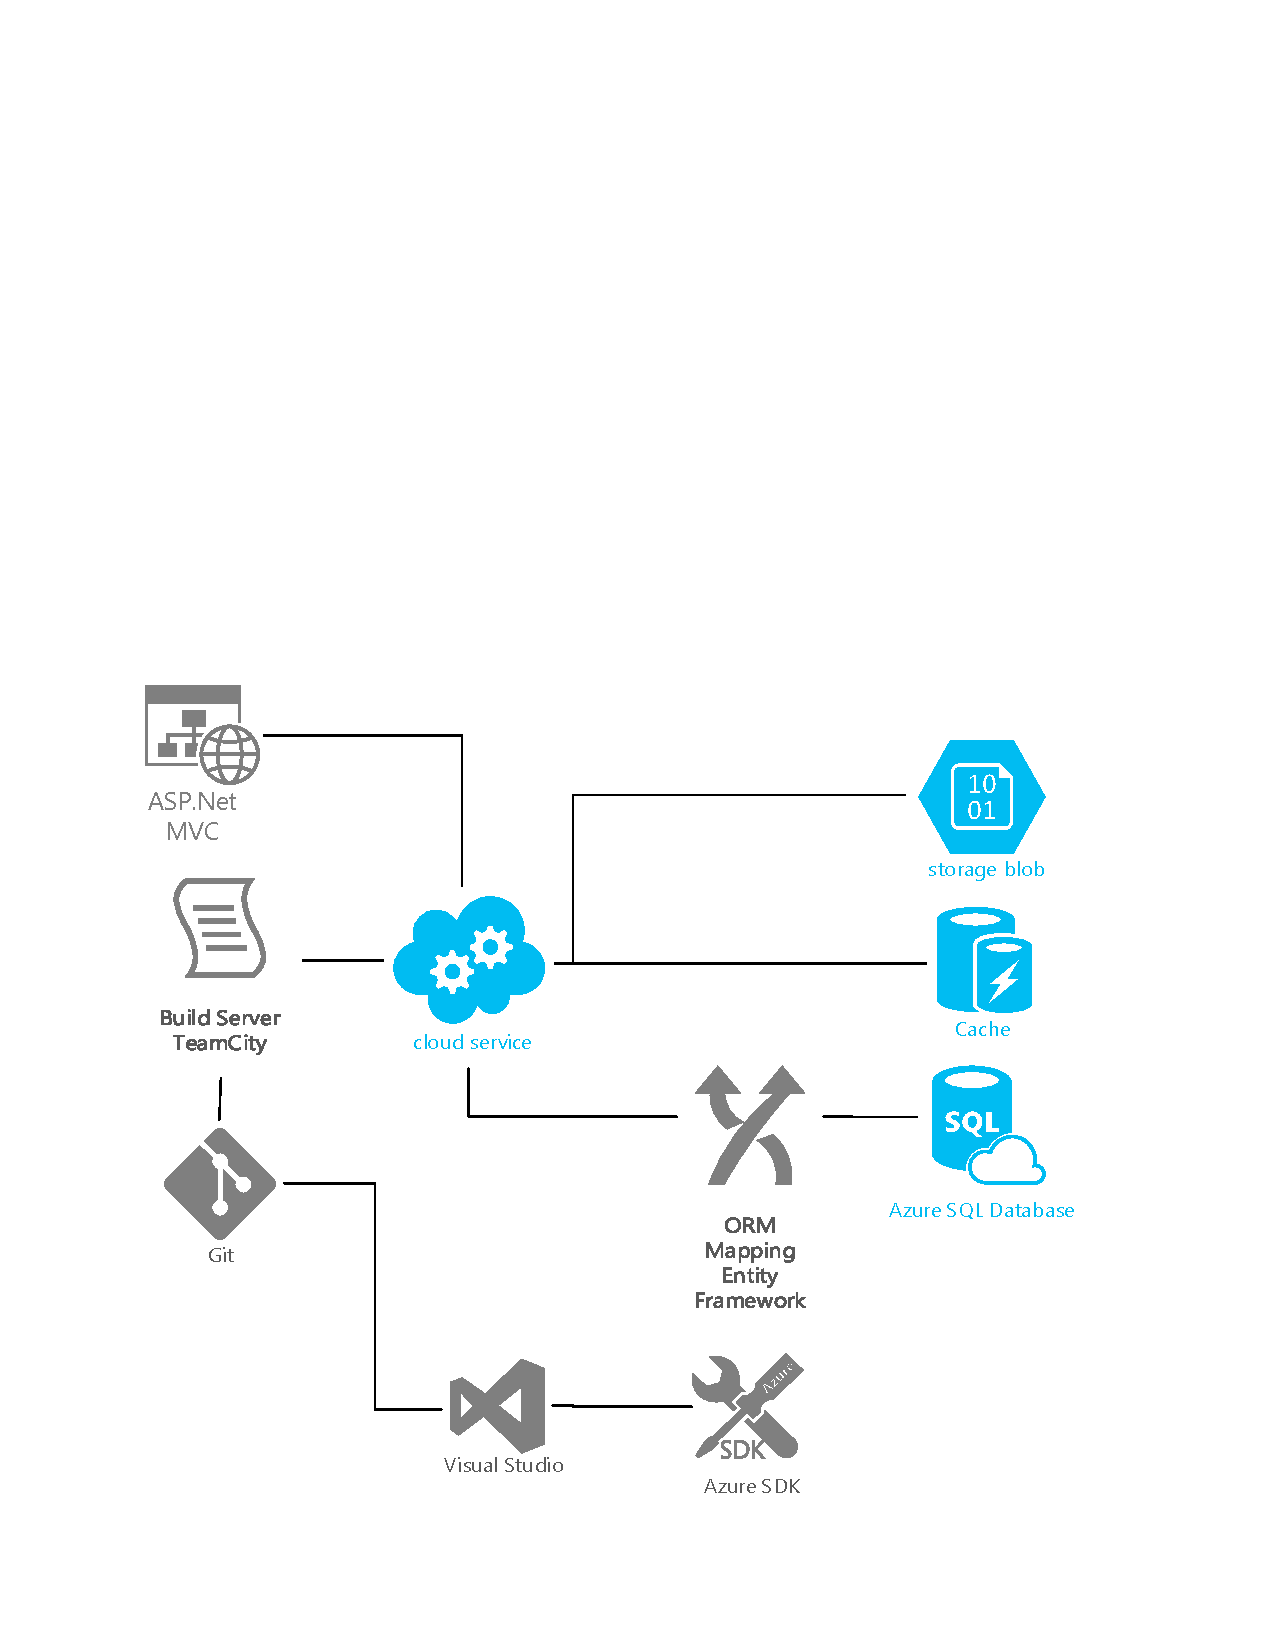
\includegraphics[width=\textwidth]{tech_breakdown}
\caption{XV Technology Breakdown}
\label{fig:tech_breakdown}
\end{figure}

The XVA was designed using the Microsoft's ASP.Net Framework. It utilizes the MVC architectural pattern for the program design and the open source Entity Framework for Object Relational Mapping (ORM) to a collection Microsoft SQL databases. Currently the application is hosted using Microsoft Azure Cloud Services. Website is hosted on Microsoft's Internet Information Services (IIS) installed on an Azure Web Role virtual machine. In conjunction with the Web Role the application uses a helper application running on an Azure Worker Role virtual machine to conduct database, email and other operational tasks. The team uses TeamCity build server for continuous integration and testing and Git and GitHub for source control. Data is persisted to two different Azure SQL Databases, firstly is the marketplace database which stores all of the application e-Commerce transaction and user data and the media database which stores all of the media specific data such as availability, pricing, form factors and publishers. The media DB is quite large (11GB) and is updated every night through the integration of different advertising data outlets and sources. The application stores large binary objects such as videos, images and sounds for the application using Azure Blob storage and uses Azure Cache in order to improve performance. XV currently does not utilize any third party components that would restrict the implementation of a multi-tenant architecture. The majority of code of the XVA was written using C\# (66.3\%) but also includes JavaScript (31.4\%) and Cascading Style Sheets (CSS) (2.1\%) for front-end design.



The application solution consists of 11 projects. The Xv.Marketplace.MVC project includes all MVC code, this includes View Models, Views and Controllers. Although conventional MVC uses models directly within the MVC application, the models for the application have been extracted into the Xv.Marketplace.Domain project. The models are presented using Plain Old CLR Object (POCO) classes combined with Data Annotations that provide the models metadata. The business logic project acts as a service layer and as the name suggest is responsible for all the business logic applied when objects are retrieved from the repositories. The Xv.Marketplace.Worker project is used to complete functional tasks that are not handled by the MVC project such as sending of emails, reminders, cleaning up of storage and indexing. The repositories project is responsible for communicating with the Microsoft SQL database and uses Entity Framework to map objects to a relational database structure and vice versa. The repositories are mostly concerned with Create, Read, Update and Delete (CRUD) operations of entities but also handle security. Finally, the Infrastructure project is used for cross cutting concerns and utilities. This includes resources used in the different projects, helper, wrapper and extension classes. All of the Test projects include either Unit tests for their corresponding projects or in the case of the repositories Test project, integration tests.


\begin{figure}
\centering
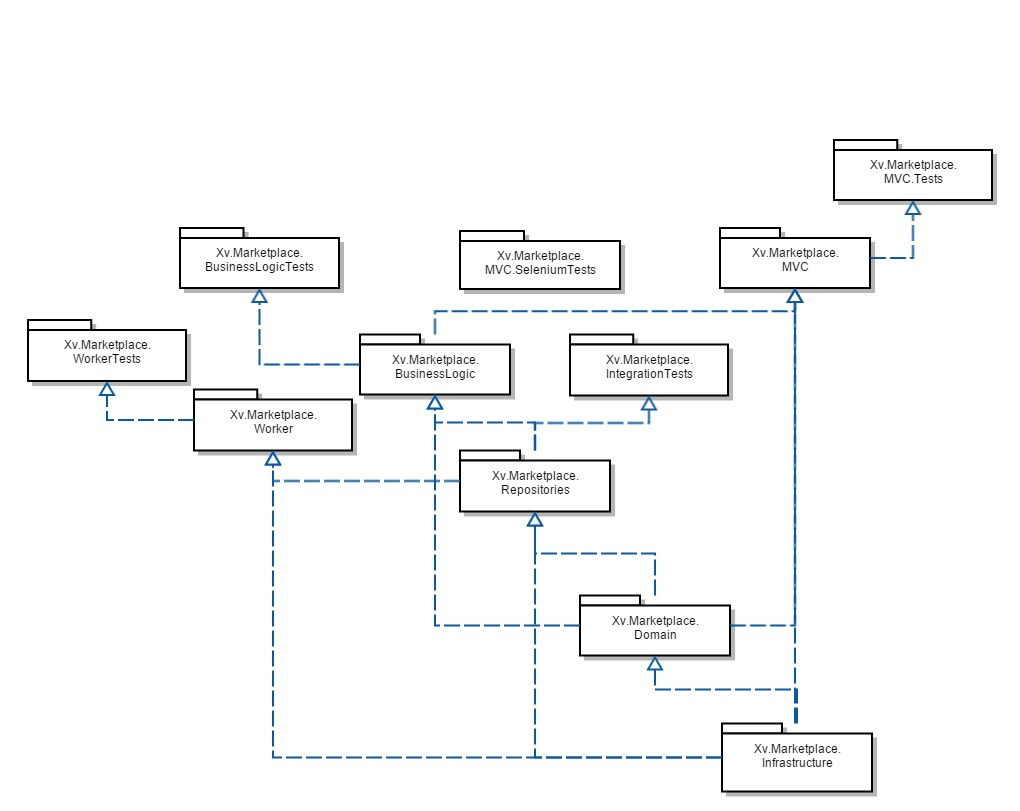
\includegraphics[width=\textwidth]{xv_proj_arc}
\caption{XV Package Diagram}
\label{fig:xv_proj_arc}
\end{figure}


\section{XVA Persistence Schemas}

As the XVA is the Core of the XV business model the exact information regarding the applications database schemas are subject to nondisclosure. In order to provide context for the case study the core tables and relationships in the marketplace database have been extracted and can be seen in Appendix \ref{fig:xv_erd}. The entity relational diagram highlights some important points about the schema used in the current application. Firstly, there is an extreme degree of denormalization used in many of the tables; this has been done in order to improve performance by grouping frequently access data together. Secondly, a lot of multi-directional relationships have developed between the entities as the schema has evolved over time. These relationships are currently a problem as entities can be accessed through multiple roots entities and the current application does not support lazy loading. This causes multiple calls to the database in order to obtain basic child objects. This greatly influences the current persistence performance



\section{Business Requirements}

In addition to the basic technical design requirements, the core business requirement for shifting to a multi-tenant model is reduction of costs. The business model also requires specific provisioning of new tenants/application customers to be streamlined and simplified in order to reduce the amount of developer time required for setting up, customizing and deploying new instances for new tenants. At the current state, provisioning of a new application customer is a long manual process within which the XV Application is manipulated and customized according to the clients' specific needs. This proved to be an extremely time consuming, expensive and resource heavy process. Therefore, one of the fundamental business requirements multi-tenant systems includes high levels of customization with low provisioning costs.

\section{Ubiquitous Language}
Domain driven design requires the establishment of a ubiquitous language in order to facilitate communication between all stakeholders and parties of a project \cite{Evans2003}. The ubiquitous language aims to minimize any assumptions and misunderstandings between stakeholders in the system.  Although this thesis does not implement DDD as an approach, it does make use of some of its principles in order to simplify eventual migration to such an approach.

Some of the definitions for the ubiquitous language include: 
\begin{itemize}
\item \textbf{Advertiser}: Person or Organization interested in advertising their own product or service through the application
\item \textbf{Publisher}: Person or Organization that has ownership of some advertising medium, for example an Private Cinema that has its own advertising space before each movie. The publisher is the person from whom the application rents its medium and is responsible for displaying the booked advertisement on the rented medium. 
\item \textbf{Manager}: XV employee responsible for handling and management of advertisements, this is primarily employees from the "Media" team. They are responsible for helping advertisers design and plan their advertising campaigns.
\item \textbf{Tenants}: Groupings of clients or specific companies that use the XV application
\end{itemize}	


\section{Conclusion}

Throughout this thesis we discuss and articulate means of which to overcome the design requirements defined by this case study. The major requirements including migrating from a SaaS maturity level 1 to a SaaS maturity level 4 implementation. Decreasing overall costs through resource sharing and simplification of the tenant provisioning process. The technological restrictions include using Windows Azure and ASP.NET MVC.
\chapter{Architecting a Multi-tenant System}
\label{chapter:architecting}
\section{Architecture \& Architecture Description} \index{Architecture Description}
This section briefly introduces concepts covered by ISO/IEC42010. It defines the terms used in the development of the architecture description artefact as well as discusses the architecture modelling language and framework used.


ISO42010 and its predecessor IEEE1471 attempted to establish a coherent practice for developing architecture descriptions, frameworks and architecture description languages \cite{InternationalOrganizationOfStandardization2011}. This in turn required the formalization and standardization of key architecting terms (see table \ref{table:iso_def} on page~\pageref{table:iso_def} for key term definitions). One of the important distinctions made by these standards was between architecture and architecture description (AD). In software architecture refers to the fundamental concepts or properties of a system, in its environment and embodied in its elements, relationships and principles of its design and evolution \cite{InternationalOrganizationOfStandardization2011}. In order to explain this architecture and its components, architects produce a product of work that helps express the architecture as a whole, namely an AD. ADs are powerful tools in expressing the core essence of a software system in relation to its key properties, behaviour, composition and evolution \cite{InternationalOrganizationOfStandardization2011}. 

Understanding this essence is also critical in helping us to bring into effect, manage and improve the system in regards to its non-functional requirements. These AD also help address known concerns of stakeholders for a system of interest \cite{Emery2009}. It is therefore an important part of any software or systems life-cycle to produce some form of architectural description to communicate different concerns to the different stakeholders from their respective views throughout. The concerns of the different stakeholders are exemplified through the use of architectural views where each view covers a set of identified concerns and is captured via the use of conceptual or meta-models \cite{42010faq}.


\section{Architecture Description Languages (ADLs)}

An ADL is a set of model, notations and specifications used that are applied in order to describe software architecture and its business domain. For this paper a few ADLs have been considered including Stanford's Rapide Project \cite{Luckham1996}, WRIGHT ADL \cite{Allen1997} and ACME \cite{bjorn}. Although ADLs are popular amongst scholars and researchers their popularity amongst architects have been questionable outside specialized domains \cite{Woods2005}. In contrast, Unified Modeling Language (UML) has seen widespread adoption by system architects. Although it is not technically considered an ADL, UML provides a set of notations that suffice for creating of general architecture description models \cite{Woods2005}.

\section{UML}

UML was adopted as the standard by the Object Management Group (OMG) in 1997. It is the result of a variety of Object-Oriented Analysis and Design methods that were introduced during the 80's and 90's \cite{Fowler2004}. Developed by a team of architects commonly referred to as the "three amigos", UML is a direct result of the work done by Grady Booch, Ivar Jacobson and James Rumbaugh at the Rational software company. After adoption as standard by OMG, UML has received widespread adoption and usage in software and enterprise systems architecture communities. UML2 includes 13 basic diagrams which are generally subdivided into two broad categories for modeling. Firstly, structural diagrams indicate static architectural constructs such as classes, objects and components as well as the relationship between these. Secondly, behavioural diagrams that are used to model the functional or dynamic constructs of an architecture. This thesis uses UML as its ADL.


\section{Architectural Framework}

ISO/IEC/IEEE 42010:2011 (ISO-42010) defines an architecture framework as "a framework establishing a common practice for creating, interpreting, analyzing and using ADs within a particular domain of application or stakeholder community".



The 4+1 Architectural View Model as designed by Kruchten \cite{Kruchten} identified five high level views for use during the creation of an AD (see figure \ref{fig:4plus1frameworksmall}). These views correspond to ISO-42010's view points as they refer to different stakeholder's views and help address these stakeholders' specific considerations. It is important to note that although \cite{Kruchten} uses the term view in his work, ISO-42010 defines the view as the physical work product of an architectural view. A simple breakdown of the 4+1 viewpoints and their mappings to supportive UML diagrams can be seen in Appendix \ref{table:viewpoints} as a composition of \cite{Muchandi2007} and \cite{Kruchten}. This thesis uses the 4+1 framework in order to define the common principles and practices for describing the architecture. This framework is combined with UML in order to provide specific viewpoints from which views are constructed via diagrams of various model types.



\section{Design Concerns in Multi-tenant Systems}
\index{Design Concern}
\index{Multi-tenant}
The architecting of any software or system faces some concerns and challenges; this is also true for multi-tenancy.\index{Multi-tenant} Although many of the challenges encountered during multi-tenant architecting is similar to that encountered in single-tenant application architecting, the challenges are often presented in another form or complexity level for multi-tenant approaches \cite{Bezemer:2010:MSA:1862372.1862393}. This section takes a look at the concerns and challenges faced when architecting a multi-tenant system and attempts to support the ultimately chosen solutions to these.

\subsection{Performance}
\label{sec:performance}
\textbf{Performance Isolation}
\\
\\
It is common for single-tenant applications to have one instance consume all available resources. In such a case one tenant's behaviour does not affect another. However, this is not the case for multi-tenant applications where resources are shared and the over-utilization by one tenant does directly impact another. Tenant performance isolation aims to reduce the performance impact between tenants through using fairness policies, throttling techniques or specific design patterns. Since multi-tenant applications aim to be elastically scalable, tenant performance isolation should be designed to support a scaling model and not restrict tenants. This means that assigning of equal amounts of resources between tenants is not an effective solution since it leads to low utilization of resources per tenant \cite{Bezemer:2010:MSA:1862372.1862393}. In order to improve performance isolation in our architecture, a Queue Centric Workflow pattern is used (see section \ref{sec:qcw}). 

\subsection{Caching}

In single-tenant applications, the use of in memory caching is a quick and easy solution to performance improvement. However, using in memory caching in a multi-tenant environment is not viable, since cached data might need to be shared across multiple application instances. In order to address this, an external cache provider has to be used for maintaining cache data for all application instances. Azure Redis Cache \index{Azure!Azure Redis Cache} is suggested for implementation in the prototype \index{Prototype} as cache provider combined with the Cache Aside pattern \cite{Homer2014}. Using an external cache instead of in memory caching does introduce some latency as a network component is introduced. As long as the application and its external cache are hosted within the same datacenter, however, this latency can be kept to an acceptable minimum.


\subsection{Scalability}
\label{sec:scalability}

\textbf{Auto-scaling}
\\
\\
Auto-scaling is the capability of dynamically allocating more or less resources as required by an application on demand and in accordance to some predefined Service Level Agreement (SLA) \cite{Homer2014}. Cloud -Native applications strive to be completely auto-scalable which allows large savings due to the over provisioning of resources. Auto-scalable applications can demand more resources be provisioned when loads are high and could allow resources to be removed when it detects that allocated resources are not being completely utilized. Although implementing a fully auto -scalable application for this thesis would be ideal, as it stands it has been deemed out of scope. However, since it is hard to change a horizontally scalable application to a completely auto-scalable one. Some architectural decisions were made with auto-scaling in mind, such as application statelessness and affinity.

\textbf{Affinity and State}
\\
\\
In order to improve the performance and scalability of our multi-tenant application, a stateless Web Tier is used. This means that the application requires no affinity, as no specific application instance will store session state data and therefore any instance can handle all application requests. This in effect allows us to scale horizontally without having to worry about maintaining affinity for our users. In cases where some session information has to be stored a client side mechanism is suggested instead. A common client side method is storing specific session data in a cookie using JavaScript Object Notation (JSON). In cases where storing sensitive information on the client side, encryption should be used. When user authentication states are stored in cookies it is also important to remember that attackers that capture the cookie will be able to impersonate that user and therefore protection mechanisms should be put in place, e.g. cross site scripting guards.


\textbf{Multi-Instance Model}
\\
\\
\label{sec:multiinstance}
\index{Multi-instance}
\index{Multi-tenant}
One major drawback introduced by migrating to a multi-tenant approach is the creation of a single point of failure. That is, that once the instance of the application goes down or is affected by some externality, all tenants are affected and are unable to access the application. If this was to occur, it could be potentially devastating for any service oriented company tied to a SLA. Therefore, some contingency for such a situation is critical to consider, even during the design phase.
 
One possible solution to help mitigate this risk is using a multi-tenant, multi-identical-instance model. That means that the exact same application and roles are replicated to different virtual machines or physical locations. A load balancer is then used to balance the load between these identical instances. In the event that something would happen to one of these instances, the load balancer would then easily be able to switch all requests to the other instance and therefore ensure the availability of the application. Azure already provides support for multi-instance models to be deployed and can be implemented using only configuration. Other multi-model supporting features commonly used include Availability sets, Fault Domains and VNets (see section \ref{sec:availability}).


\subsection{Security}
\label{sec:security} 

\textbf{Dual Input/Tenant Validation (DITV)}
\\
\\
\label{sec:ditv}
User authentication in a multi-tenant system requires additional security measures. Firstly, users need to be authenticated in order to ensure that they are allowed to access the application. Once a user has been authenticated against the service, they need to be authenticated against the tenant they are claiming to belong to. Only once a tenant has been authenticated to both use the system and access a specific tenant's data is it allowed to be fully authenticated. Furthermore, user requests also need to be checked to ensure they are allowed to be executed against the requested tenant. This forms part of tenant data isolation.


\textbf{Tenant Data Isolation}
\\
\\
One of the primary risk factors introduced by multi-tenancy is that of "cross tenant data leakage". An example of this is a case where a CRUD command of one tenant affects or retrieves the information of another tenant. For any application this is behaviour would be unacceptable. It is therefore that proper tenant data isolation is considered one of the essential security factors that needs to be addressed by the systems architect \cite{Wilder2012-so}. By using DITV authentication queries can be analyzed and adapted in order to ensure that they only retrieve information connected to the requested tenant and by an authorized customer.


\subsection{Availability}
\label{sec:availability}
\index{Availability}
In order to control the physical hosting location for your services, Azure requires you to bind your services to a specific region. This region corresponds to the (currently 11) available Azure Data Centres around the world\cite{Microsoft_Corporation2014-bf}. Specifying which region should host your services is equal to selecting the actual data centre where your services will be physically hosted. However, within the data centre it might be beneficial to co-locate services in close physical proximity to each other in order to reduce latency, up performance and cut costs \cite{Microsoft_Corporation2014-dn}.
 

This is where affinity groups come into play. These groups are defined at subscription level and helps Azure to know to group services that belong to a specific affinity group in close physical proximity. Affinity groups are tied to regions.
 
It is important to note that with recent changes in Azure Virtual Network structures that the VNets are no longer tied to affinity groups, but directly associated with the regions. This means that when you create your VNet and affinity group, they should both be located in the same region \cite{Microsoft_Corporation2014-dn}.

\subsection{Configuration and Customization}
\label{sec:custandconf}

The degree to which individual customers are able to customize anything from layouts to schemas should be carefully considered during the application design stages in order to ensure that the architecture allows for sufficient customization from the start. Krebs states that the ability to handle different tenant specific configurations regarding User Interface (UI) as well as other functional, or non-functional behaviour can be considered as key enablers for multi-tenant applications \cite{Krebs2012}. Since tenants will require some changes or modifications such as extended features, implementation of these features should not influence other parts of the system.
 
The customization required by our multi-tenant application proves to be one of the core elements driving many of the design choices. Each tenant requires complete customization of the front-end to fit their respective Corporate Identity (CI) as well as lower level extension to the system such as publisher filtering on database level. This essentially means specific publishers should only be shown to specific tenants, and some to all. Other important customization considerations include workflow processes used by different clients and how workflows would be implemented to include possible changes by the client.


\textbf{Tenant Customization}
\\
\\
\label{sec:viewengine}
In many multi-tenant systems the difference between tenants is minor and can usually be handled by storing the differences in configuration. Settings such as Corporate Identity (CI), which includes fonts, colours and logos, as well as workflow that have been enabled or disabled, is retrieved from the external configuration and applied. However, in our system, this level of configuration is not enough. The XVA requires high levels of modification for the front-end for each tenant. Although the development of highly configurable software is not commonly the responsibility of the multi-tenant application \cite{Krebs2012}, the specific of implementing such an application has been considered during the architecture design. As such, custom views are a robust solution for implementing tenant specific customizations. Custom views effectively allow us to create different views for each tenant, customizing the HTML and CSS for that view to the tenant's requirements. It also allows us to create a custom master or layout view that can be used to apply the tenants CI. This solution could also allow us to use shared views for situations where tenant specific customization is not required. In order for our custom view solution to be applied in ASP.NET \index{ASP.NET} MVC,\index{Model View Controller (MVC)} we create a custom view engine. View engines are primarily responsible for rendering the code from your views into HTML that is served by the browser.

However, View Engines are also capable of defining search paths and retrieving specific views to be served. It is these capabilities that are used to allow our application to search for, and retrieve tenant specific views. Since our requirement does not include any customization to the way views are rendered, extending an existing view engine such as Razor is the most viable option. Morris \cite{Morris} provides a good example implementation of such an extended Razor view engine that allows for multi-tenancy. His approach is implemented in the prototype. A major drawback of using custom views is it removes our ability to dynamically provision new customized tenants. If the tenant's configuration is stored separately from the system following the external configuration store pattern, \cite{Homer2014} new tenants can be provisioned dynamically without any modified views. However, since adding views to a project requires the project to be rebuilt, a new deployment will have to be made when custom views are added. For our case, however, the high customizability provided by custom views outweighs the drawback of having to constantly redeploy. In order to ease the influence of constant redeployments, using of a continuous integration workflow is strongly suggested.


\subsection{Maintenance}
\label{sec:maintainance}
Bezemer \& Zaidman \cite{Bezemer:2010:MSA:1862372.1862393} state that using multi-tenancy could result in a maintenance dream since application deployment is significantly simplified. By using a single instance of the application and database, any changes simply need to be deployed once. However, this simplified maintenance is closely coupled with implementation quality. High quality multi-tenant application utilize a layered architecture that has multi-tenancy applied as a cross cutting concern \cite{Bezemer:2010:MSA:1862372.1862393}.


\textbf{Provisioning}
\\
\\
Since adding tenant specific views requires redeployment, provisioning of new tenants with their custom views in our system will not be an automated process. Tenants can, however, be created dynamically as tenant data is stored externally. This means new tenants can be provisioned without a redeploy, but will only have the generic shared or default views set. In order to properly provision a new custom tenant, however, the tenant's specific views can firstly be created, a deployment done and once the tenant needs to be activated it can be created dynamically by an application manager. Once the tenant's data has been stored, the application will then be able to automatically associate the custom views with that tenant and start serving the tenant specific customized views. This provisioning process works for our specific case study since a new tenant is usually slowly introduced and requires such high levels of view customization. Multi-tenant systems that have large numbers of tenants (10+) should however rather consider moving away from the custom views into a more generic configuration based customization approach, especially where tenant provisioning should be completely dynamic and automated. One method helping to reduce the impact of redeployment for tenant provisioning is by using a build server such as TeamCity combined with a continuous deployment, integration and delivery strategy.


\subsection{Persistence Design}

In multi-tenant system design, many different approaches to designing a persistence model can be taken including \cite{Krebs2012}:

\begin{itemize}
\item Dedicated database: Each tenant has their own specific database. This approach offers the highest level of tenant isolation, but is considered the least effective multi-tenant approach since it does not attempt to share resources. Allows the high levels of schema customization per tenant.
\item Dedicated table/schema: Tenants share a single database, but have their own dedicated tables within that database. This approach is considered better at resource sharing, but still does not allow high enough levels of resource sharing. Cross tenant queries for reporting purposes are also harder to implement with this approach. Furthermore, this approach allows high degrees of schema customization.
\item Shared table/schema: All tenants share a single schema or table and provide means for schema extension through extension columns. This approach is considered the purest multi-tenant approach, but implores restrictions on schema modification.
\end{itemize}


Since our application requires a constantly varying schema, using a schema-less database has been chosen. This allows us to obtain the highest degree of flexibility. In order to allow the most effective persistence design to be implemented, a shared database, dedicated collection approach was taken. This approach is similar to the dedicated table/schema approach in the sense that a single database is used by all tenants, but each tenant has their own respective collection (groupings of documents, searchable indexes, entities, etc.). Furthermore since a single data storage type does not fit all our specific needs, such as auto-indexing of fields for searchable items and easy persistence of JSON objects as query-able documents, a polyglot persistence\index{Polyglot persistence} model is used.


\textbf{Polyglot Persistence Model}
\\
\\
The term polyglot persistence is used to refer to the utilization of different data stores and types in order to store data \cite{Sadalage2012-zw}. This means that systems information is stored in various different databases with different schemas and models in order to be used for their intended purpose and by providing the required benefits for that specific data storage type. For this thesis, a polyglot persistence approach is taken by storing specific data into different databases and different database types. Media items that should be searchable, quickly queried and should have powerful search and filtering features such as geo-search are stored in Azure Search \index{Azure!Azure Search} (Database). This allows all media items to use an easily modifiable schema (at code level), while providing full text search and fully indexed objects for quick and constant queries. The marketplace data is stored in Azure Document DB \index{Azure!Azure Document DB} since the document storage is fast and easy to use. It allows more complex querying compared to key-value store typed storage and allows us to persist objects directly into the database without the need to use an ORM mapper. Finally for identity information, traditional Azure SQL is used since this works well with existing identity providers and have been optimized to work out of the box such as Open Web Interface for.NET (OWIN). Stateful data such as a user's shopping cart or selected media items is stored using Azure Cache and client side cookies. This specific separation of persistence allows us to gain the benefits of each of the respective persistence technologies at the cost of introducing higher code complexity.


\subsection{Accessibility}

One of the most common ways to distinguish between tenants is using the tenant's name as area and mapping the tenant name as an area using MVC routing. However, XV tenants wish to maintain their own Domain Name System (DNS) names and access to the system should therefore be setup using sub domains. A suggested method for doing this is setting up a Canonical Name Record (CNAME) entry with our DNS provider that points all domains via the "*" wildcard to the application instance. This will allow us to have tenants to set up their DNS to point to <tenant-name>.<our-domain>.


\section{Conclusion}
This chapter took a look into the Architecture Description standard for Systems and software engineering outlined by ISO4210. It also introduced the Architecture Framework used to present our description, namely the 4+1 View Model. Finally, it discusses a combination of common high level design concerns encountered in multi-tenant and cloud applications and possible ways of addressing them. 
%\chapter{Cloud Architecture Design Patterns}
\label{chapter:patterns}
This chapter introduces different design patterns that were used in Chapter \ref{chap:ad}. It aims to provide some background on the chosen patterns and justify their requirement. A short description of how these patterns are applied in the prototype \index{Prototype} is also provided as well as relevant technologies used in conjunction.

\section{Cloud Design Patterns \& Multi-tenancy}
\index{Multi-tenant}

A fundamental decision in any software and system architecture venture is choosing appropriate design patterns. Wilder \cite{Wilder2012-so} defines design patterns as an approach that can be duplicated in order to produce an exact and expected outcome. One of the most referenced definitions of a pattern is by Alexander et. al which states that a pattern describes a problem that occurs over and over in our environment, and then describes the core of the solution to that problem in such a way that you can use the solution a million times over, without ever doing it the same way twice \cite{Alexander1977-ni}. In order to address some of the requirements of the system and help solve some problems that are introduced by using a multi-tenant approach, implementation of some design patterns are necessary. Some of these problems include addressing scalability, handling server load spikes and variations tenant isolation. 

\textit{Note: The selection of these patterns are a result of a modified Attribute-Driven Design Approach (see section \ref{sec:add}) and qualitative interpretation of its results (see section \ref{sec:arcdrivers}).}

\section{Eventual Consistency}

Brewer's cap theorem, although a common misnomer \cite{Brewer2012}, is often used to justify the implementation of eventual consistency using NoSQL over traditional Relational Database Management Systems (RDBMS ) \cite{Wilder2012-so}. Distributed cloud systems have embraced the idea of eventual consistency since preventing downtime is of higher importance than providing consistent data. In many applications, it is acceptable to serve somewhat stale data as long as the application continues to run even in case of node failures. The concept of eventual consistency states that although the system attempts to be consistent, there is a short tolerated delay in consistency which exists while data updates gets propagated \cite{Wilder2012-so}. Since it is important for our system to remain online and working even in the case of node failure and at the cost of consistency an approach that favours availability has been taken in the choosing of design patterns to apply. The system will also attempt to adhere to the Basically Available, Soft State and Eventually Consistent (BASE) guarantees over the Atomicity, Consistency, Isolation and Durability (ACID) guarantees.
 
 
\section{Command Query Responsibility Segregation (CQRS)}
\index{Command Query Responsibility Segregation (CQRS)}
 
CQRS is a popular design pattern used in scalable cloud based applications. At its core, the pattern is defined as a separation between the queries (data requests) operations and commands (data modification) \cite{Homer2014}. This stands in contrast to traditional CRUD operations that are all handled together using the same model or entity. The argument for separating these operations includes reduced complexity of domain models, increased scalability and simplification of implementation \cite{Homer2014}. Scalability is improved by allowing read and write stores to be scaled independently depending on usage. Implementation is simplified and performance is improved since views can be composed according to View Models and data can be de-normalized in order to improve queries. Although the pattern does not implicitly require the separation of data stores, it is useful to consider for building cloud-native applications. 
 
CQRS embraces the fact that consistency of data is given up in order to provide better availability \index{Availability} and partitioning and therefore does not try to solve the problems of stale data. Instead, it explicitly understands that data is stale and would be updated to be eventually consistent. The CQRS pattern is commonly used in conjunction with Event Sourcing in order to construct a write only stream of commands that are executed to modify the data \cite{Homer2014}. However, due to the complexities involved with setting up a complete event subscriber/publisher workflow around the Event Sourcing pattern, a Queue Centric Workflow pattern has been used as a alternative. Another advantage of CQRS is it significantly simplifies the need for transformations of models between layers since the query operations could select related view data directly into View Models without needing to transpose the other layers. In its essence, CQRS works with the fact that if you try to optimize a single domain object for both commands and queries, it would become bloated and ineffective at either. In the system we attempt to implement CQRS (without Domain Driven Design (DDD)) by clearly separating the workflow of our commands and queries, including separation of models all the way through to repositories. Figure \ref{fig:CQRSFlow} shows the high level breakdown of application layers and query vs. command workflow. One of the major obstacles in implementing CQRS, however, is the fact that since commands are processed independently from queries, commands cannot return the modified object \cite{Homer2014}. This means that users should be notified that their command has been queued for execution but they cannot be guaranteed to see the results immediately. Instead alternative mechanisms might be considered in order to notify users that their commands have been processed such as SignalR push technologies. This is also an extremely important fact to mind during UI design.
 
 
\section{Queue Centric Workflow}
\label{sec:qcw}
\index{Queue Centric Workflow}
 Queue Centric Workflow (QCW) patterns describe a method for loosely coupling requests between the presentation layer and lower application layers as seen in figure \ref{fig:CQRSFlow}. A common problem with SaaS \index{Software as a Service (SaaS)} implementations is its unpredictable loads \cite{Homer2014}. In multi-tenant applications this becomes an even bigger issue as spikes in usage from one tenant directly impact other tenants \cite{Betts2012-ad}. In order to isolate tenants from the impacts of load spikes, a QCW based load levelling pattern has been implemented. The pattern describes the introduction of a queue between tasks and services that run asynchronously \cite{Wilder2012-so}. A task posts a message into a queue that contains all required data relevant to its execution. A service then retrieves these messages and processes them at a consistent rate. This allows the queue to act as a buffer protecting the service from becoming flooded and affected too dramatically by load spikes.
It is also possible to scale the service that processes queue messages in order to handle increased queue loads. In our project we considered using an Azure Worker Role (see appendix \ref{appendix:azure}) to be setup as a service that consumes our queued tasks and executes them. However, due to the lower costs and ease of implementing Azure WebJobs compared to worker roles this option was used for demonstration purposes instead. Migration between these two Azure services is extremely simple and required minimal modification if it would be required for production implementation. The prototype uses the CQRS workflow as seen in figure \ref{fig:CQRSFlow}. A Console Application that is hosted as WebJob runs continuously and consumes messages from Azure Storage Queues (see appendix \ref{appendix:azure}). The presentation layer creates tasks in the form of commands that is posted to the queue and then executed in a consistent manner by the WebJob.
 
\begin{figure}
\centering
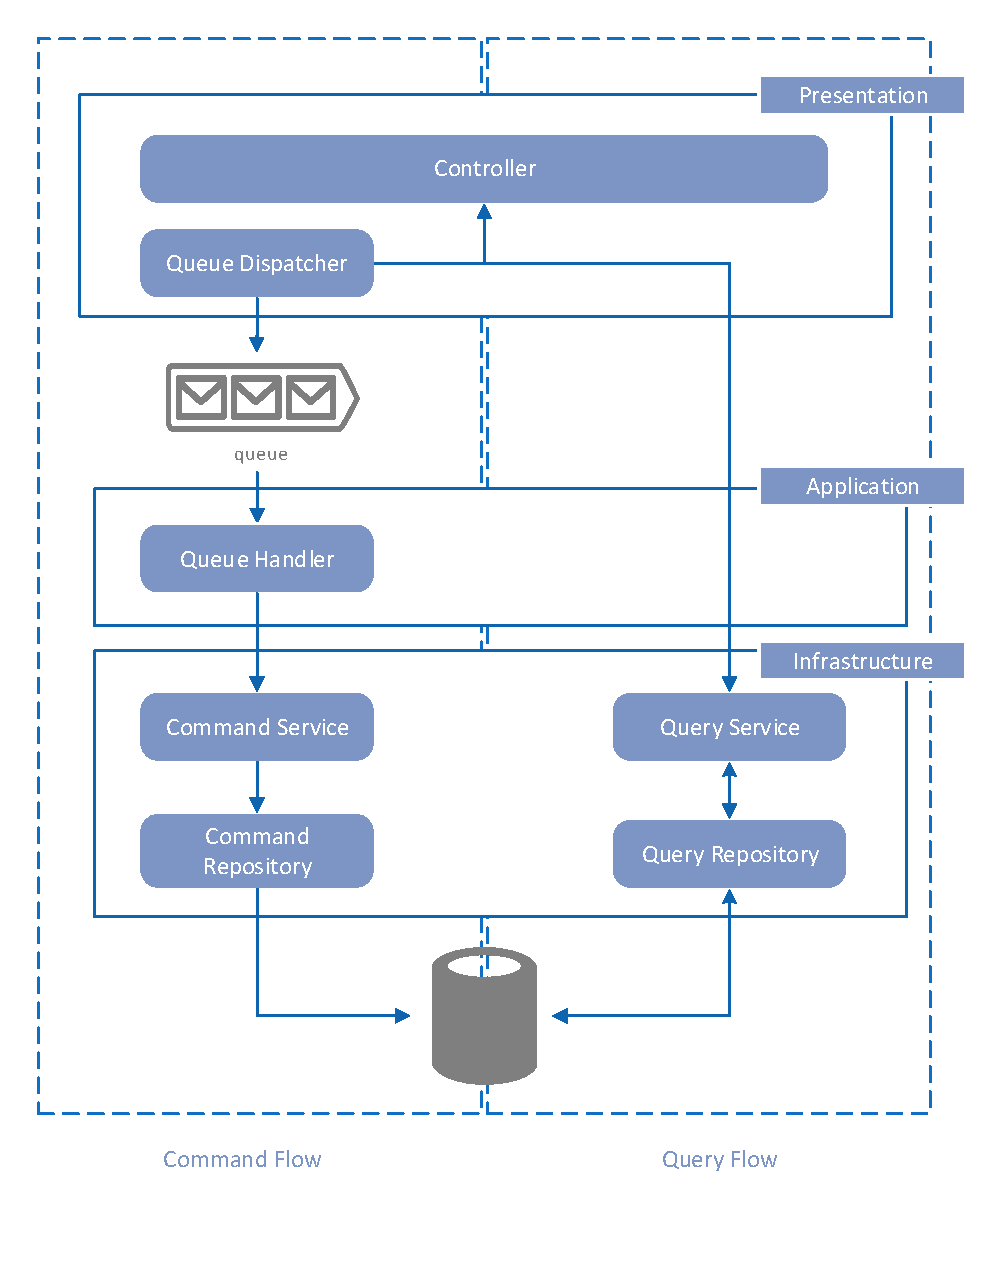
\includegraphics[width=\textwidth]{CQRSFlow}
\caption{CQRS, QCW and Command pattern work flow}
\index{Command pattern}
\label{fig:CQRSFlow}
\end{figure}
 
 
 \section{Command Pattern}
 
 The command pattern uses a uniform interface that isolates execution data from the invoker. This is achieved by exposing only an execute method that when called, handles delegation of the requests' implementation to other objects \cite{Gamma1994-ho}. The command pattern is useful when combined with other patterns such as CQRS, Event Sourcing and especially with QCW patterns. The command pattern also allows us to create specific command objects that represent real world business cases and helps move more to DDD. Command objects are also useful as they encapsulate all the information required for delayed execution, \cite{Gamma1994-ho} which is central to queue or message based implementations. In our prototype, the command pattern is used to encapsulate all modifications to data in our data stores. The controllers create command objects and then pass these into a queue via our queue service. A worker role/WebJob that constantly queries the queue picks up these commands and then invokes their execute method. This way our presentation layer never executes any commands and contains no references to our command repositories or services. It simply uses the queue service to line up commands for execution. This separation of command implementation from command invocation can help us create a highly scalable system based on eventual consistency.
 
 
 \section{Cache Aside Pattern}
  \label{sec:cache}
 Application performance can be significantly improved by implementing a caching solution. By using a cache, an application reduces the amount of calls to its data stores and instead reads commonly used data from memory. Instead of using persistent storage to hold data, caches are usually implemented in memory, and these significantly increase its read and write speeds. However, cached data needs to be constantly maintained in order to ensure consistency. One pattern that helps with solving the consistency issue between the data store and the cache is the Cache Aside pattern. This is a very simple pattern that describes using three basic steps in order to ensure cache data is updated \cite{Homer2014}:
 
    \begin{enumerate}
        \item On query request, check if the item is currently in the cache
        \item If the item is in the cache, return the cached version
        \item If the item is not in the cache, retrieve it from storage and save it to the cache
   \end{enumerate}
   
 
On command requests the object in the cache should be invalidated in order to be retrieved again on its next query request. For this thesis, the Cache Aside pattern is used in combination with Azure Redis Cache.\index{Azure!Azure Redis Cache} Updates are handled by the service objects. Any queries retrieve the data from its respective storage and then serializes it and adds it to the cache. Any command deletes the cached item with the key corresponding to the changed entity id.


\section{Conclusion}
 
Multi-tenant applications introduce new problems that are solvable by certain design patterns outlined here. Firstly, the problem of tenant isolation can be addressed through application of a QCW pattern or more precisely, a queue based load levelling pattern. This QCW pattern is further extended by applying the command pattern, effectively turning tasks into self-containing objects that could be queued up for later execution. The problem of scalability is addressed by implementing the QCW as it allows commands to be lined up and handled asynchronously in the background. This alone, however, is not enough to be considered truly cloud-native and scalable. In order to ensure easy scalability, the CQRS pattern is introduced. This pattern helps to separate all query operations from command operations, all the way down to the models.
 
This combined with a QCW allows the application to easily scale its command processing by provisioning more instances of the queue handler. Similarly, it also provides the ability for the query processing through provisioning of more read only data stores to be accessed. These patterns are used in conjunction with the Cache Aside pattern by storing data in the cache on query operations and deleting them on command operations. This provides overall improved performance. Instead of attempting to ensure consistency in the system, availability is considered higher priority and thus allows the implementation of these patterns in ensuring the BASE guarantees are met.
%\chapter{Amalgamating Design Inputs, Patterns and Concerns}
This chapter uses an modified Attribute-Driven Design approach to attempt to bring all the design inputs and discussions from the previous chapters together. It aims to provide  design patterns and approaches that address specific design concerns \index{Design Concern} that have been extracted from the functional requirements, \index{Functional Requirements} quality attributes and design constraints.\index{Design Constraint}

\section{Adapted Attribute-Driven Design Approach}
 \label{sec:add} 
In creating an architecture description,\index{Architecture Description} the architect is faced with a range of diverse approaches. Each one of these approaches offers a certain framework for creating the AD and sets certain context and constraints on the design used. One such comprehensive approach to AD design is Attribute-Driven Design (ADD). In its essence, ADD is an approach to defining an AD that uses the software's quality attribute requirements as baseline for the design process \cite{Wojcik2006}. This approach uses an iterative, recursive process to attempt to decompose a system into elements by applying architectural tactics and patterns \cite{Wojcik2006}. The ADD approach provides highly detailed ADs that should satisfy all of the system requirements and quality attributes. This thesis uses a simplified and broad-viewed approach based on ADD in the creation of its architecture description. It does not attempt to completely follow ADD, but instead uses the ADD recommended process as blueprint for creation of the AD.

\section{System Requirements and Constraints}
\label{sec:reqandconstraints}
The following requirements and constraints have been defined after analysis of the use case, literature on multi-tenancy and recommendations of various stakeholders. Table \ref{tab:quality_attributes} outlines the quality attributes that need to be satisfied by our architecture (see Chapter 2, 6, 7). Whereas table \ref{tab:functional_requirements} specifies the core functional requirements for our media marketplace  (see Chapter 4) and table \ref{tab:design_constraints} addresses the constraints placed on our architecture  (see Chapter 4). 


\subsection{Quality Attributes}
\begin{table}[!h]
\centering
\begin{tabularx}{\linewidth}{|l|X|l}
\cline{1-2}
QAR1 & The system shall be scalable under variable tenant loads &   \\
QAR2 & The system shall be highly available in cases of failures &    \\
QAR3 & The system shall be modifiable in terms of adding new tenants &    \\
QAR4 & The system shall be performing normally under variable tenant loads &    \\
QAR5 & The system shall be secure in isolating tenant data &    \\
QAR6 & The system shall be usable in configuring the system to tenant specific requirements &    \\
\cline{1-2}
\end{tabularx}
\caption{Quality Attribute Requirements (QARs) in Priority Order}
\label{tab:quality_attributes}
\end{table}
\newpage

\subsection{Functional Requirements}
\begin{table}[!h]
\centering
\begin{tabularx}{\linewidth}{|l|X|l}
\cline{1-2}
FR1 & The system shall allow the creation of new tenants dynamically with default views &   \\
FR2 & The system shall allow custom views to be deployed per tenant &    \\
FR3 & The system shall allow managers to add basic configuration info for a tenant &    \\
FR4 & The system shall allow users to create a campaign with specific to and from dates &    \\
FR5 & The system shall allow users to query for available advertising media &    \\
FR6 & The system shall allow users to add selected media to a campaign &    \\
FR7 & The system shall allow users to book campaigns &   \\
FR8 & The system shall allow managers to view booked campaigns and approve or deny them &  \\
FR9 & The system shall allow users to view the status of their booking &   \\
FR10 & The system shall allow media to be searched based on geographic point &   \\
FR11 & The system shall plot available media on a map according to the media's geographic point &   \\
\cline{1-2}
\end{tabularx}
\caption{Functional Requirements (FR) in Priority Order}
\label{tab:functional_requirements}
\end{table}
\newpage

\subsection{Design Constraints}
\begin{table}[!h]
\centering
\begin{tabularx}{\linewidth}{|l|X|l}
\cline{1-2}
DC1 & The system shall be implemented using technologies that are either openly and freely available or provided by the BizSpark program &   \\
DC2 & The system shall be hosted on Windows Azure using either Azure Websites or Azure Web roles combined with either Azure WebJobs or Azure Worker Roles &  \\
DC3 & The system shall be implemented using C\# &    \\
DC4 & The system  shall use the .NET 4.5 framework    \\
DC5 & The system shall use ASP.NET \index{ASP.NET} MVC for its front-end &    \\
\cline{1-2}
\end{tabularx}
\caption{Design Constraints (DC) in Priority Order}
\label{tab:design_constraints}
\end{table}

\index{Model View Controller (MVC)}

\subsection{Quality Attribute Scenarios}
In accordance to ADD, each Quality Attribute outlined in table \ref{tab:quality_attributes} should be expressed in a stimulus-response form similar to quality attribute scenarios. As such, each QAR has been explicitly broken down from table \ref{table:qar1}, page \pageref{table:qar1} to table \ref{table:qar7} on page \pageref{table:qar7}. These scenarios provide a good stimulus-response breakdown for our quality attributes and allows us to measure the effectiveness of our AD against them. These scenarios are also used in selection of patterns and creation of system elements.

\section{System Elements Decomposition}
After assessing the requirements inputs, quality attribute scenarios and use case further, a broad-overview breakdown of the system has been done into four major container elements. This breakdown is outlined in figure \ref{fig:elements}. Each element could be further defined as follow:
\begin{itemize}
\item \textbf{Presentation}: This element is concerned with providing the front-end to our system using ASP.NET MVC and other web technologies. The presentation element should be modifiable by nature allowing it to be altered according to tenant needs and specifications. This element will also include all marketplace related functionality
\item \textbf{Application}: The application element provides background processing and functionality and should be tenant neutral. It is concerned with the back end functionality requirements
\item \textbf{Persistence}: The persistence element is concerned with the storage, retrieval and modification of application data. This includes all service and repository functionality
\item \textbf{Infrastructure}: The infrastructure element contains the components, models and other elements concerned with cross cutting concerns. This element forms part of and is used by all other elements
\end{itemize}

\begin{figure}
\centering
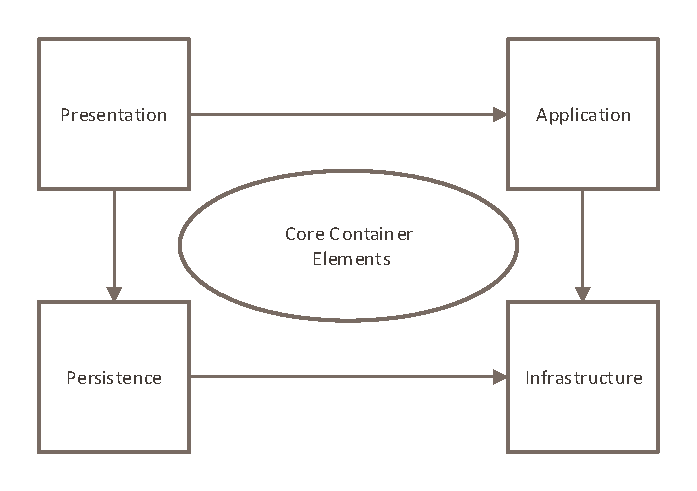
\includegraphics[width=\textwidth]{CoreElements}
\caption{Architecture Core Container Elements}
\label{fig:elements}
\end{figure}


\section{Architectural Drivers}
\index{Architectural Driver}
 \label{sec:arcdrivers}
An analysis of the architectural drivers for each element was made following the techniques outlined by Wood \cite{Wood2007}. This analysis can be seen in appendix \ref{table:architecturaldrivers}. Each requirements is analysed in accordance to its importance and impact or difficulty of implementation. This creates a combination of priorities as outlined by the case study and qualitative interpretation of research conducted. These priorities are then used to select the highest importance, highest impact drivers to architect first. 

\subsection{Candidate Architectural Drivers (CAD)}
Using the architectural drivers and their priorities, all requirements that have a direct influence on the architecture (high and medium impact) have been mapped to each element as shown in figure \ref{fig:designconcernmapping}. This mapping not only allows us to identify the CADs but also indicated three shared requirements amongst all elements nl. QAR1, QAR2 and DC2. These three requirements in effect form three shared concerns that hold a high priority.


\begin{figure}
\centering
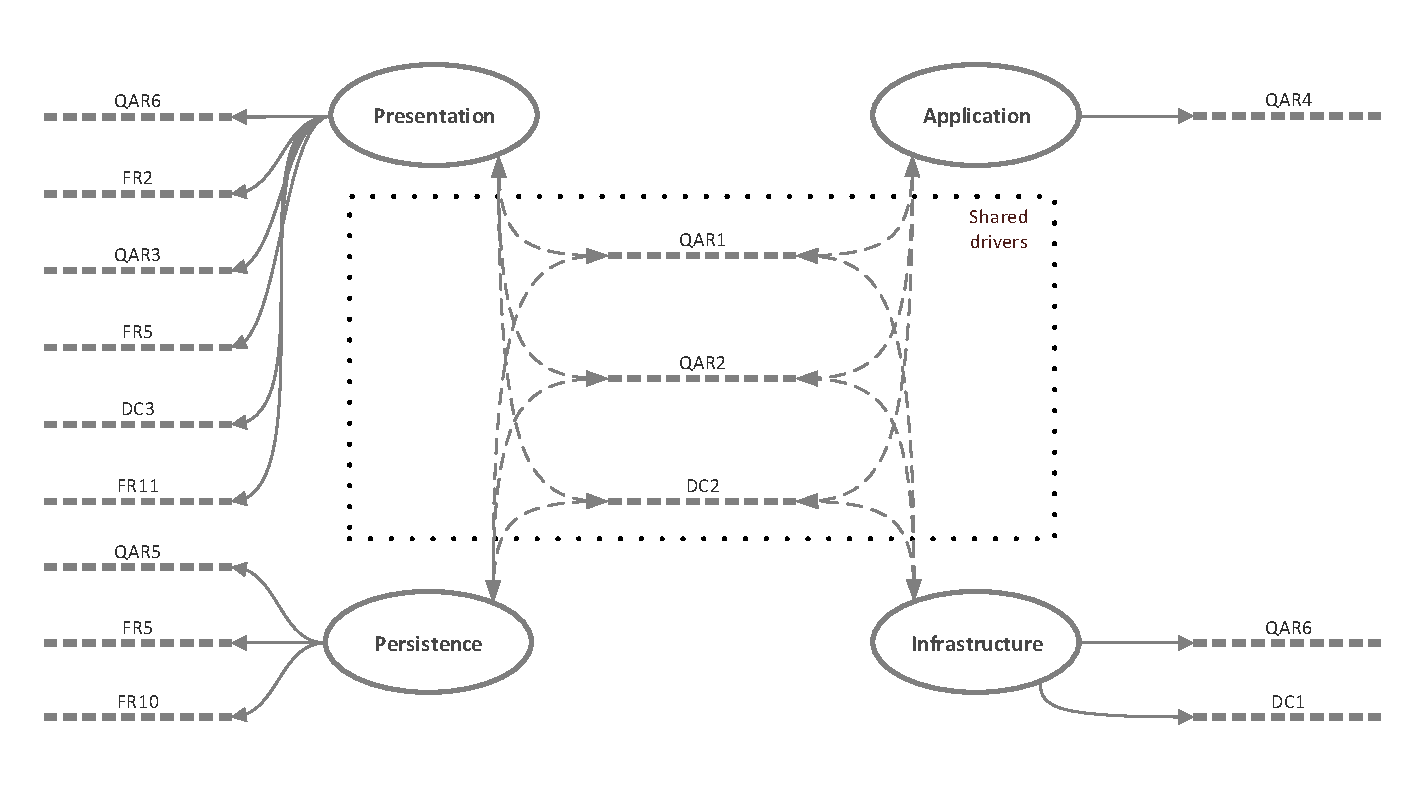
\includegraphics[width=\textwidth]{DesignDriverBreakdown}
\caption{Candidate Architectural Drivers Mapping}
\label{fig:designconcernmapping}
\end{figure}

\section{Design Concerns}
\label{sec:designconcerns}
The mapping of candidate architectural drivers seen in figure \ref{fig:designconcernmapping} further allows us to separate requirements that have a direct impact on our architecture from those that do not. After filtering out these requirements, each CAD can be connected to a specific architectural concern as described in Chapter \ref{chapter:architecting} Architecting a Multi-tenant System. By doing this mapping, specific requirements are grouped together into specific concerns. Furthermore, these concerns indicate specific problems that needs to be addressed by our AD as well as the effectiveness of the solution. These requirements are also used as perspective in selecting appropriate architectural design patterns to use in the resolution of each concern. See table \ref{table:designconcerns} for the resulting mappings. 


\begin{table}[h]
\centering
\begin{tabularx}{\linewidth}{lXl}
\rowcolor[HTML]{EFEFEF} 
\begin{tabular}[c]{@{}l@{}}Candidat\\ Architectural\\ Driver\end{tabular} & \begin{tabular}[c]{@{}l@{}}Design\\ Concern\end{tabular} & \begin{tabular}[c]{@{}l@{}}Related\\ Sections\end{tabular} \\
QAR1 & Scalability & \ref{sec:scalability} \\
QAR2 & Availability & \ref{sec:availability} \\
QAR6 & Configuration \& Customization & \ref{sec:custandconf} \\
FR2 & Configuration \& Customization & \ref{sec:custandconf} \\
QAR3 & Maintenance & \ref{sec:maintainance} \\
QAR5 & Security & \ref{sec:security} \\
QAR4 & Performance & \ref{sec:performance} \\
DC1 & Technical Constraint & \ref{sec:techconst} \\
DC2 & Technical Constraint & \ref{sec:techconst} \\
\end{tabularx}
\caption{Driver, Concern and Related Section Mappings}
\label{table:designconcerns}
\end{table}

One important aspect to note from the concerns outlined in table \ref{table:designconcerns} is the Environment concern. This specific concern does not require the application of any design patterns as it simply implies some limitations on the technologies that could be used. The following breakdown of technologies have been selected according to this concern (for more information on each of these technologies see appendix \ref{appendix:azure}):
\begin{itemize}
\item \textbf{Web platform}: Azure Cloud Services - Web Role (web server) and Worker Role (background processing)
\item \textbf{Web server}: Internet Information Services (IIS)
\item \textbf{Cache}: Azure Redis Cache
\item \textbf{Persistence}: Azure Document DB, Azure Search,\index{Azure!Azure  Search} Azure SQL \index{Azure!Azure Document DB}
\item \textbf{Queue}: Azure Storage Queues
\item \textbf{Logging and Debugging}: Elmah, Application Insights
\end{itemize}

\section{Design Concerns and Suggested Approaches}
In order to address each one of the concerns outlined in table, \ref{table:designconcerns} different patterns have been evaluated. The term pattern used in this section refers to the definition by Alexander \cite{Alexander1977-ni}. As a result, the term patterns describes any of the following system architecture patterns, design patterns, cloud architecture patterns, workflow patterns and even specific sub-types of patterns of any of the above. In essence, the patterns chosen have been a result of the qualitative interpretation of research done for this paper, personal experience \& skills as well as recommendations from various online sources. In addition, the CQRS pattern has been examined specifically for its viability, as members of XV has expressed direct interest in implementing it. 

\subsection{Maintenance Concern}
Implementation of multi-tenancy is the primary principle that is applied to simplify maintenance. Since the current XV platform requires modification of several application instances and uses a different code base for each tenant. Its deployment process is overly complex. It is therefore that this principle will help address this concern. However, implementing multi-tenancy introduces other maintenance issues. In our case, QAR3/4 (see table \ref{table:qar3}) requires that the system be maintainable in terms of adding new tenants. By using the suggested View Engine solution  discussed in section \ref{sec:viewengine}, we can remove many of the complexities of implementing custom views for tenants. Using a custom view engine will allow us to simply create new views that will overwrite global ones for each tenant. Although many pure multi-tenant solutions suggest using an approach where all customisation and configuration for tenants is done through configuration, our solution will not allow this. Tenants for our case require extreme degrees of front-end customisation and are provisioned on a monthly basis. This slow provisioning time allows us to use the custom view engine approach instead of using a pure customisation through configuration one. Additionally, the layering pattern has been chosen to help improve maintainability as well. Implementing the layering pattern allows us to decouple our system into different layers or tiers, each responsible for a specific grouping of functions. In contrast to the existing layering pattern implemented in XVA, a layering pattern that utilises the layers suggested by DDD will be used instead. The primary justification for using DDD layering is XV's attempt to migrate towards a more domain driven architecture. This decision is also coupled with implementing CQRS.


\subsection{Availability Concern}
\index{Availability}
No patterns were selected that directly influence our availability concern. Since Azure already implements various availability assurance mechanisms and their SLA provides terms for high availability, this concern has minimal impact on the architecture implementation. However, for the Azure High Availability SLA to apply, we are required to host at least two instances of any of our components. This corresponds to the multiple-instance model suggested for addressing the scalability concern (see section \ref{sec:multiinstance}). Implementation of availability sets, should be used to ensure redundancy and remove the impact of planned or unplanned maintenance events as well as failures. Specific application elements will be grouped into an availability set. These availability sets simply assure that our grouped instances are in separate update domains. This ensures that only one instance of our components will ever be shut down at a time for updates. Azure also automatically deploys application instances to different fault domains. This ensures that hardware failure should affect only one instance of the application and never all of them. 


\subsection{Scalability Concern}

In order to address the scalability requirements of our system, many different patterns have been reviewed. The patterns that have been ultimately selected include: load balancing, auto-scaling, command query responsibility segregation, command pattern and queue centric workflows. The advantages and disadvantages of CQRS, Command and QCW \index{Queue Centric Workflow} patterns have also been outlined in table \ref{tab:scalability_patterns}. These patterns primarily allow scalability by decoupling the system components and allowing easy, horizontal scaling through adding more instances. These instances could be any part of the system. Since a combination of CQRS, \index{Command Query Responsibility Segregation (CQRS)} QCW and the command pattern \index{Command pattern} is used, our presentation layer should be completely independent of executing any commands itself. This has the advantage of being able to scale up the web tier in cases of high query loads. In cases where there is a high command load more instances of the queue handler or application tier can be provisioned. Similarly the query database (if different query and command stores are used) could also be scaled horizontally. Using Azure technologies as required by [DC1/2] allows us to do this scaling on the fly and allows for scaling by metric (see appendix \ref{appendix:azure}). This means that scaling could be setup to be handled automatically and be elastic. The multi-instance\index{Multi-instance} approach is also what will primarily be used for addressing our availability concern. These specific patterns were selected due to their relevance as cloud architecture patterns. The CQRS pattern, although criticised as merely a trending pattern, has seen widespread acclaim by various system architects. This is especially true where implemented in combination with DDD. This pattern also directly addresses some of the issues with scaling for multi-tenancy through clean separation of query and command concerns. The QCW pattern is commonly used as supportive pattern to CQRS as it allows an even further degree of separation between the presentation, application and persistence elements. Implementation of this pattern allows independent scaling of, any of our application elements. The command pattern has been chosen to implement in combination with the other two as it allows delayed execution of commands and helps us to separate the front end from understanding any execution logic. This in effect allows us to move all business or domain logic to the application layer. It also allows us to queue commands to remove concurrency problems. Finally, using the auto-scaling pattern has also been considered. The auto-scaling pattern however has not been included in table \ref{tab:scalability_patterns} as it will be used, but not be implemented by our system. This is due to the fact that Windows Azure already implements different auto-scaling strategies that can be enabled purely through configuration.  


\subsection{Configuration and Customisation Concern}
The External Configuration Store Pattern is used to address the Configuration and Customisation Concern. This pattern simply states that configuration information should be store outside of the application files. Using this approach allows us to centralise configurations for all different instances of our application and its components. Although this pattern refers specifically to application configuration, we will use this pattern to apply to tenant configuration as well. The External Configuration Store pattern suggests the implementation of a management back-end that can be used to manipulate configuration that is separated from the core application.

\subsection{Security Concern}
Since multi-tenancy requires additional security considerations, especially in terms of isolation between tenants, selecting an appropriate approach is quite difficult. In order to address this concern, an modified version of input validation is suggested (see section \ref{sec:ditv}). This method uses multi-facet authentication. Firstly a user is authenticated normally with input validation checks. Once a user has been authenticated, all requests the user issues are checked to see if they originate from a valid tenant domain. Once it has been established that a request comes from a valid domain, the user is checked against the tenant that the domain belongs to. This ensures that only users that have been authorized for specific tenants can execute commands on that tenant. Only after this dual input/tenant validation has been done, requests processed. Using this approach also allows us to dynamically include the tenant that the requests originated from into each command or query. Thus, allowing us to further apply filtering or query adaption mechanisms. This tenant level filtering can be applied in the persistence element, effectively only allowing queries and commands to be executed for the tenant they originate from. 


\subsection{Performance Concern}
The performance and scalability concerns in our system are highly interlinked. Since many of the features used to achieve scalability also allow for improved performance and vice-versa. The primary performance pattern that has been chosen is the cache aside pattern. This pattern has been discussed in section \ref{sec:cache}. This pattern basically allows us to have an external cache provider that has entries added on queries and deleted on commands. Additional patterns and approaches that help address this concern include:

\begin{itemize}
\item Load Balancing: Allows loads to be shared between instances. Achievable through Azure Load Balancer and for region wide balancing Azure Traffic Manager
\item Denormalization: Reduces the amount of joins required to retrieve commonly used entities by grouping them together. Achievable through NoSQL and Azure Document Database
\item Content Delivery Networks: Allows commonly accessed data to be stored closer to users via distributed CDNs. Achievable by using Azure CDN
\end{itemize}

\subsection{Resulting Patterns, Approaches and Configurations}
The results of the discussions of section \ref{sec:designconcerns} has been summarised in figure \ref{fig:concernpatterns}. It indicates the different patterns and approaches applied, as well as patterns that can be implemented via configuration in Windows Azure.


\begin{figure}
\centering
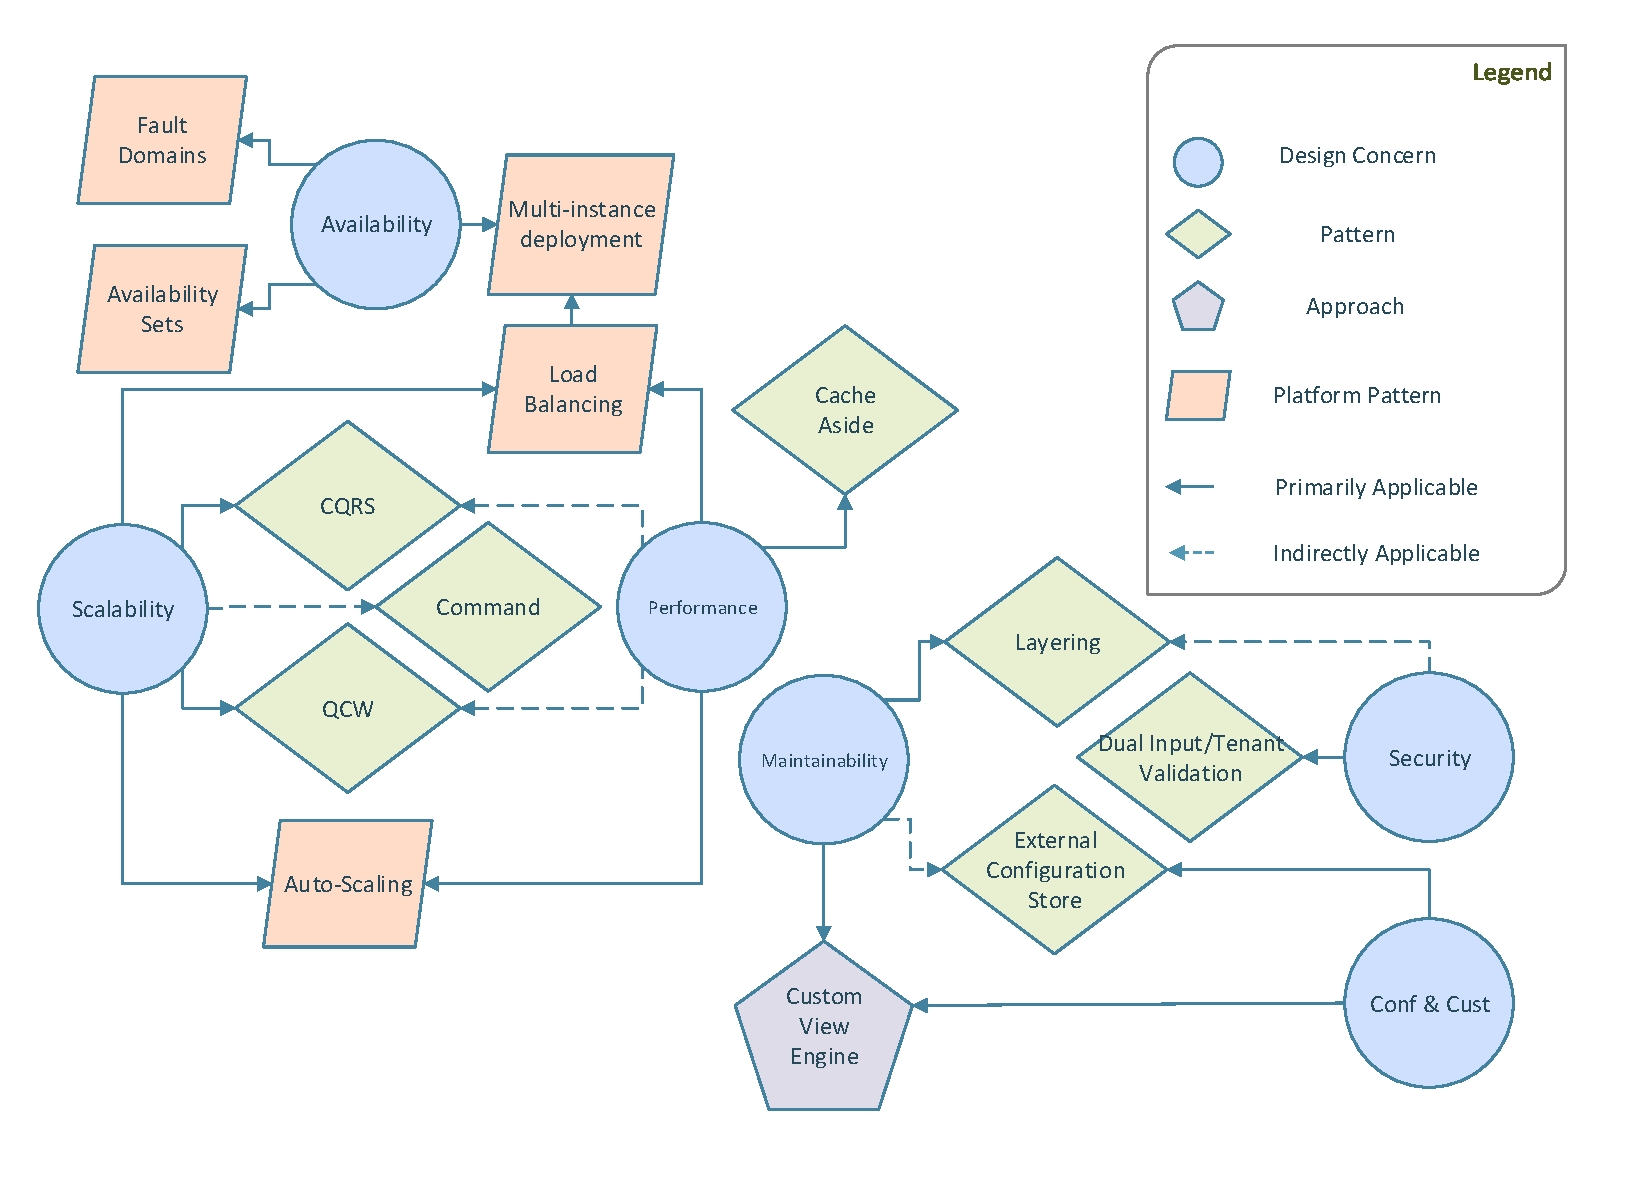
\includegraphics[width=\textwidth]{ConcernPatterns2}
\caption{Design Concerns, Patterns, Approaches and Configurations}
\label{fig:concernpatterns}
\end{figure}

\section{Conclusion}
This chapter brought together chapters 2 through 6. It uses ADD as an guideline for refining our functional requirements, design constraints and quality attributes into specific design concerns. It then supports the selection of patterns and approaches that are applicable to addressing these design concerns and summarises them in figure \ref{fig:concernpatterns}. Which is used as baseline for the creation of many of the diagrams in the following chapter. 
%\chapter{Prototype Artefact - XVP}

In order to measure the viability of the produced architecture description artefact a prototype artefact has been created. This artefact, codenamed XV Prototype (XVP) is used in order to gain valuable implementation insights into the development of an actual working multi-tenant application. It also helps reflect on architectural decisions made and provides useful feedback for improvement of the architecture development for future production implementations.

\section{Application Source Code}

The source code for our prototype has been hosted on BitBucket and is accessible from \textbf{https://bitbucket.org/auronmatrix\_/xvp}. Please note that the repository is private as the source code contains some sensitive and private information. \textbf{To obtain access to this repository please send your requests to 417457@mail.muni.cz}

\section{Accessing the Prototype}
For this project the domain fithesis.info was registered and an a CNAME (Alias) entry was added to the DNS Zone File to point all hosts (*) to our azure instance (xvp.azurewebsites.net). This allows us to dynamically add any tenants with their own custom domain name in the form
<custom-subdomain>.fithesis.info. 

Two core tenants have been setup:
\begin{itemize}
\item ao.fithesis.info (default) : Primary tenant, representing the XV site with full functionality
\item xv.fithesis.info (custom tenant) : Secondary tenant with custom layout, views and workflows
\end{itemize}

\section{Tenant Provisioning}
When a new tenant is created without a redeployment with customized views the view engine will automatically access the shared default views and use them. Once custom views have however been created and a redeployment done the view engine will retrieve these custom views in priority order:
\begin{enumerate}
\item tenant-<tenant-name>/controller
\item tenant-<tenant-name>/shared
\item global/controller
\item global/shared
\end{enumerate}

\section{Limitations and Issues}
\subsection{Azure Pricing}
In contrast to implementing the prototype on Windows Azure Web Roles and using Azure Worker Role instances, it was decided to implement the prototype using Azure Websites and Azure WebJobs instead. In Appendix \ref{appendix} these technologies and their respective advantages disadvantages are discussed. This problem is considered low impact since it does not alter a lot of code. However, the physical performance of this choice is noticeable.

\subsection{Domain Driven Design}
CQRS is commonly implemented as pattern in conjunction with domain driven design \cite{Swanson}. This leads to a radical change in the way domain objects are created and the way they act. It also requires using of aggregates for accessing related entities. Fundamentally, completely implementing domain driven design would be ideal since it would give us the many of the domain driven design benefits. As such it is recommended for any further implementations of a system based on the prototype to use domain driven design as its principal design approach. However, in order to simplify the design, creation and implementation processes, domain driven design has not been implemented in the prototype. Also since existing team members are not completely familiar with DDD and its specifications from a business perspective this choice made sense. In order for the application to be easily migrated to a DDD approach the DDD application layers have been used in the prototype implementation already. This plus CQRS and the Command pattern allows us to easily switch to a DDD approach by removing the generic command objects and replacing them with domain specific commands.

\subsection{WebJob Polling Service}
An Azure WebJob application is used to consume and execute commands placed in the Azure Storage Queue. The WebJob works very efficiently for processes that require long running asynchronous background processing. Since we implement CQRS and the majority of commands in the storage queue is related to data persistence operations (insert, update, delete) which although not time critical, is time sensitive. With the Azure WebJobs setup the WebJobs only polls the storage queues once every 10 minutes by default. This value has been changed to under 10 seconds however a small delay in time the command is queued and time the command is executed can still be observed. The easiest solution to this problem would require moving out of the Azure Websites as WebJob and into their own respective Azure Worker Role instance. This would significantly improve the performance of the queue handler as Worker Roles run as their own application instances with dedicated memory, where WebJobs run within an Azure Website with shared memory. This would also allow us better flexibility in the configuration of the application environment and would allow us to optimize the instance for processing messages from the storage queue.

\subsection{Azure Document Db Preview Release Limits}
At time of writing Azure Document DB has only been released for Public Preview. Specific limitations that severely affected the prototype development and method for implementing multi-tenancy was its container limitations \cite{AzureLimits}. Each DocumentDB only allows the creation of 3 collections that act as containers for documents. This proved to be a problem since a collection per tenant approach for specific information and a shared container approach for others was used by our architecture description. In order to solve the container problem, database level separation (as opposed to container) level separation was implemented. However this introduces severe limitations on cross tenant querying capabilities and should not be followed in the production implementation.

\section{Conclusion}


%\chapter{Prototype Artefact - XVP}
\index{Prototype}

In order to measure the viability of the produced architecture description \index{ Architecture Description} artefact, a prototype artefact has been created. This artefact, codenamed XV Prototype (XVP) is used in order to gain valuable implementation insights into the development of an actual working multi-tenant \index{Multi-tenant} application. It also helps reflect on architectural decisions made and provides useful feedback for improvement of the architecture development for future production implementations.

\section{Application Source Code}

The source code for our prototype has been hosted on BitBucket and is accessible from \textbf{https://bitbucket.org/auronmatrix\_/xvp}. Please note that the repository is private as the source code contains some sensitive and private information. \textbf{To obtain access to this repository please send your requests to 417457@mail.muni.cz}

\section{Accessing the Prototype}
For this project, the domain fithesis.info was registered and a CNAME (Alias) entry was added to the DNS Zone File to point all hosts (*) to our azure instance (xvp.azurewebsites.net). This allows us to dynamically add any tenants with their own custom domain name in the form
<custom-subdomain>.fithesis.info. 

Two core tenants have been setup:
\begin{itemize}
\item ao.fithesis.info (default) : Primary tenant, representing the XV site with full functionality
\item xv.fithesis.info (custom tenant) : Secondary tenant with custom layout, views and workflows
\end{itemize}

\section{Tenant Provisioning}
When a new tenant is created without a redeployment with customized views the view engine will automatically access the shared default views and use them. Once custom views have however been created and a redeployment done the view engine will retrieve these custom views in priority order:
\begin{enumerate}
\item tenant-<tenant-name>/controller
\item tenant-<tenant-name>/shared
\item global/controller
\item global/shared
\end{enumerate}

\section{Limitations and Issues}
\subsection{Azure Pricing}
In contrast to implementing the prototype on Windows Azure Web Roles and using Azure Worker Role instances, it was decided to implement the prototype using Azure Websites and Azure WebJobs instead. In Appendix \ref{appendix} these technologies and their respective advantages disadvantages are discussed. This problem is considered low impact since it does not alter a lot of code. However, the physical performance of this choice is noticeable.

\subsection{Domain Driven Design}
CQRS \index{Command Query Responsibility Segregation (CQRS)} is commonly implemented as pattern in conjunction with domain driven design \cite{Swanson}. This leads to a radical change in the way domain objects are created and the way they act. It also requires using of aggregates for accessing related entities. Fundamentally, completely implementing a domain driven design would be ideal since it would give us the many of the domain driven design benefits. As such, it is recommended for any further implementations of a system based on the prototype to use domain driven design as its principal design approach. However, in order to simplify the design, creation and implementation processes, the domain driven design has not been implemented in the prototype. Also since existing team members are not completely familiar with DDD and its specifications from a business perspective, this choice made sense. In order for the application to be easily migrated to a DDD approach the DDD application layers have been used in the prototype implementation already. This plus CQRS and the Command pattern \index{Command pattern} allows us to easily switch to a DDD approach by removing the generic command objects and replacing them with domain specific commands.

\subsection{WebJob Polling Service}
An Azure WebJob application is used to consume and execute commands placed in the Azure Storage Queue. The WebJob works very efficiently for processes that require long running asynchronous background processing. Since we implement CQRS and the majority of commands in the storage queue is related to data persistence operations (insert, update, delete) which although not time critical, is time sensitive. With the Azure WebJob setup, the WebJob only polls the storage queues once every 10 minutes by default. This value has been changed to under 10 seconds, however, a small delay in the time a command is queued and it is executed can still be observed. The easiest solution to this problem would require moving out of the Azure Websites as WebJob and into their own respective Azure Worker Role instance. This would significantly improve the performance of the queue handler as Worker Roles run as their own application instances with dedicated memory, where WebJobs run within an Azure Website with shared memory. This would also allow us better flexibility in the configuration of the application environment and would allow us to optimise the instance for processing messages from the storage queue.

\subsection{Azure Document Db Preview Release Limits}\index{Azure!Azure Document DB}
At time of writing Azure Document DB has only been released for Public Preview. Specific limitations that severely affected the prototype development and method for implementing multi-tenancy \index{Multi-tenant} was its container limitations \cite{AzureLimits}. Each DocumentDB only allows the creation of 3 collections that act as containers for documents. In order to solve the container problem, database level separation (as opposed to container) level separation was implemented. However this, introduces severe limitations on cross tenant querying capabilities and should not be followed in the production implementation.

\section{Conclusion}


\printbibliography{}
\printindex
\appendix
\chapter{Tables}

\section{4+1 Mapping}
\begin{sidewaystable}[h]
\centering
\begin{tabularx}{\textwidth}{X X X X}
\hline
\rowcolor[HTML]{C0C0C0} 
\multicolumn{1}{|X|}{\cellcolor[HTML]{C0C0C0}\textbf{Viewpoint}} & \multicolumn{1}{X|}{\cellcolor[HTML]{C0C0C0}\textbf{Stakeholder}} & \multicolumn{1}{X|}{\cellcolor[HTML]{C0C0C0}\textbf{Description}}                                                                                                              & \multicolumn{1}{X|}{\cellcolor[HTML]{C0C0C0}\textbf{Applicable Model Types (UML)}}                             \\ \hline
\multicolumn{1}{|X|}{Logical view}                               & \multicolumn{1}{X|}{End-Users}                                    & \multicolumn{1}{X|}{Breakdown of the objects or parts of a system. It describes the functionality to be provided to the end-users}                                             & \multicolumn{1}{X|}{Class Diagrams, State Diagrams, Object Diagrams, Sequence Diagrams,Communication Diagrams} \\ \hline
\multicolumn{1}{|X|}{Process view}                               & \multicolumn{1}{X|}{Administrators and Managers}                  & \multicolumn{1}{X|}{Provides information on the workflow of objects into processes in order to explain the run-time behaviour of the system and how its processes communicate} & \multicolumn{1}{X|}{Activity Diagram}                                                                          \\ \hline
\multicolumn{1}{|X|}{Physical view}                              & \multicolumn{1}{X|}{System Engineer, Architect, Developer}        & \multicolumn{1}{X|}{Overview of the physical hardware and software the system is composed of, how they are arranged (topology) and how they communicate.}                      & \multicolumn{1}{X|}{Deployment Diagram}                                                                        \\ \hline
\multicolumn{1}{|X|}{Development view/ Implementation view}      & \multicolumn{1}{X|}{Developer, software Engineers}                & \multicolumn{1}{X|}{Provides overview of project structure from programming viewpoint including libraries, packages and run-time environments}                                 & \multicolumn{1}{X|}{Component Diagram, Package diagrams}                                                       \\ \hline
\multicolumn{1}{|X|}{Use case viewpoint/ Scenario viewpoint}     & \multicolumn{1}{X|}{All stakeholders}                             & \multicolumn{1}{X|}{Functional requirements of the system broken down into scenarios that indicate uses of the system by its stakeholders}                                     & \multicolumn{1}{X|}{Use Case Diagrams}                                                                         \\ \hline
                                                                 &                                                                   &                                                                                                                                                                                &                                                                                                               
\end{tabularx}
\caption{4+1 Viewpoint to UML Mapping}
\label{table:viewpoints}
\end{sidewaystable}



\section{ISO Definitions}
\begin{table}[h]
\centering
\begin{tabularx}{\textwidth}{|p{2.5cm}|X|l}
\cline{1-2}
\cellcolor[HTML]{C0C0C0}\textbf{Term} & \cellcolor[HTML]{C0C0C0}\textbf{Definition}                                                                                                                                              &  \\ \cline{1-2}
Architecting                          & Process of conceiving, defining, expressing, documenting, communicating, certifying proper implementation of, maintaining and improving an architecture throughout a system's life-cycle &  \\ \cline{1-2}
Architecture                          & Fundamental concepts or properties of a system in its environment embodied in its elements, relationships, and in the principles of its design and evolution                             &  \\ \cline{1-2}
Architecture Description (AD)         & The work product used to express an architecture                                                                                                                                         &  \\ \cline{1-2}
Architecture Framework                & Conventions, principles and practices for the description of architectures established within a specific domain of application and/or community of stakeholders                          &  \\ \cline{1-2}
Architecture View                     & Work product expressing the architecture of a system from the perspective of specific system concerns                                                                                    &  \\ \cline{1-2}
Architecture Viewpoint                & Work product establishing the conventions for the construction, interpretation and use of architectural views to frame specific system concerns                                          &  \\ \cline{1-2}
Architectural Concern                 & Interest in a system relevant to one or more of its stakeholders                                                                                                                         &  \\ \cline{1-2}
Environment                           & context determining the setting and circumstances of all influences upon a system                                                                                                        &  \\ \cline{1-2}
\end{tabularx}
\caption{ISO 42010 Definitions}
\label{table:iso_def}
\end{table}
\newpage


\section{Quality Attribute Scenarios}
\begin{table}[h]
\centering
\begin{tabularx}{\linewidth}{|
>{\columncolor[HTML]{EFEFEF}}l |X|l}
\cline{1-2}
\multicolumn{2}{|l|}{\cellcolor[HTML]{C0C0C0} Scalability: System loads requires scaling horizontally} &  \\ \cline{1-2}
Element & \cellcolor[HTML]{EFEFEF}Scenario &  \\ \cline{1-2}
Stimulus & 

Requires specific nodes/components to accommodate more users 
& \\ \cline{1-2}
Source & 

System owner 
& \\ \cline{1-2}
Environment & 

Normal Operation, Heavy System Loads 
&  \\ \cline{1-2}
Artefact & 

Specific system node/component 
& \\ \cline{1-2}
Response & 

Scale specific node/component horizontally for duration of the heavy load and scale back once load is reduced below certain threshold 
&  \\ \cline{1-2}
Measure & 

Scale by metric 
&  \\ \cline{1-2}
\end{tabularx}
\caption{QAR1 Scenario}
\label{table:qar1}
\end{table}

\begin{table}[h]
\centering
\begin{tabularx}{\linewidth}{|
>{\columncolor[HTML]{EFEFEF}}l |X|l}
\cline{1-2}
\multicolumn{2}{|l|}{\cellcolor[HTML]{C0C0C0} Availability: Application Node Failure} &  \\ \cline{1-2}
Element & \cellcolor[HTML]{EFEFEF}Scenario &  \\ \cline{1-2}
Stimulus & 

System node/component has a fault 
& \\ \cline{1-2}
Source & 

Fault (External or Internal), Datacenter failure
& \\ \cline{1-2}
Environment & 

Normal, Datacenter Maintenance, Degraded System Mode
&  \\ \cline{1-2}
Artefact & 

System 
& \\ \cline{1-2}
Response & 

In event of one of the system component failures all operations should be directed to alternative running instances. System should spin up new instances if required 
&  \\ \cline{1-2}
Measure & 

Downtime interval 
&  \\ \cline{1-2}
\end{tabularx}
\caption{QAR2 Scenario}
\label{table:qar2}
\end{table}

\begin{table}[h]
\centering
\begin{tabularx}{\linewidth}{|
>{\columncolor[HTML]{EFEFEF}}l |X|l}
\cline{1-2}
\multicolumn{2}{|l|}{\cellcolor[HTML]{C0C0C0} Modifiability: Adding Tenants} &  \\ \cline{1-2}
Element & \cellcolor[HTML]{EFEFEF}Scenario &  \\ \cline{1-2}
Stimulus & 

Wants to add a tenant to the system without custom views
& \\ \cline{1-2}
Source & 

Tenant Manager, Administrator, Developer
& \\ \cline{1-2}
Environment & 

Normal operations on Front-end
&  \\ \cline{1-2}
Artefact & 

System 
& \\ \cline{1-2}
Response & 

The system adds the new tenant to the tenant data and allows the tenants domain to access the system using the default views 
&  \\ \cline{1-2}
Measure & 

Effort to add tenant 
&  \\ \cline{1-2}
\end{tabularx}
\caption{QAR3 Scenario}
\label{table:qar3}
\end{table}


\begin{table}[h]
\centering
\begin{tabularx}{\linewidth}{|
>{\columncolor[HTML]{EFEFEF}}l |X|l}
\cline{1-2}
\multicolumn{2}{|l|}{\cellcolor[HTML]{C0C0C0} Tenants performance isolation} &  \\ \cline{1-2}
Element & \cellcolor[HTML]{EFEFEF}Scenario &  \\ \cline{1-2}
Stimulus & 

Utilizes a large number of resources or load creates a load spike
& \\ \cline{1-2}
Source & 

Tenant
& \\ \cline{1-2}
Environment & 

System under high loads
&  \\ \cline{1-2}
Artefact & 

System and Services
& \\ \cline{1-2}
Response & 

Other tenants should not be noticeably affected by a single tenants increased loads. Little to no impact on front-end responsiveness 
&  \\ \cline{1-2}
Measure & 

Front-end latency
&  \\ \cline{1-2}
\end{tabularx}
\caption{QAR4 Scenario}
\label{table:qar4}
\end{table}


\begin{table}[h]
\centering
\begin{tabularx}{\linewidth}{|
>{\columncolor[HTML]{EFEFEF}}l |X|l}
\cline{1-2}
\multicolumn{2}{|l|}{\cellcolor[HTML]{C0C0C0} Modifiability: Adding Tenants with Custom Views} &  \\ \cline{1-2}
Element & \cellcolor[HTML]{EFEFEF}Scenario &  \\ \cline{1-2}
Stimulus & 

Wants to add a tenant to the system with custom views
& \\ \cline{1-2}
Source & 

Tenant Manager, Administrator, Developer
& \\ \cline{1-2}
Environment & 

Normal operations on Front-end
&  \\ \cline{1-2}
Artefact & 

System
& \\ \cline{1-2}
Response & 

The developers create custom views that correspond to the tenants requirements and do a redeployment, after QAR3 is executed the system should then use the custom views over the default views for the tenant with the specified tenant configuration
&  \\ \cline{1-2}
Measure & 

Effort of provisioning new tenant with custom views
&  \\ \cline{1-2}
\end{tabularx}
\caption{QAR5 Scenario}
\label{table:qar5}
\end{table}

\begin{table}[h]
\centering
\begin{tabularx}{\linewidth}{|
>{\columncolor[HTML]{EFEFEF}}l |X|l}
\cline{1-2}
\multicolumn{2}{|l|}{\cellcolor[HTML]{C0C0C0} Security: Tenant Data Isolation} &  \\ \cline{1-2}
Element & \cellcolor[HTML]{EFEFEF}Scenario &  \\ \cline{1-2}
Stimulus & 

Wants to ready tenant specific data from the respective data store
& \\ \cline{1-2}
Source & 

Tenant Advertisers, Tenant Managers
& \\ \cline{1-2}
Environment & 

Normal operation
&  \\ \cline{1-2}
Artefact & 

System and System Data
& \\ \cline{1-2}
Response & 

The system should isolate other tenant data and ensure that no unauthorized access to other tenants data is made and no modifications of other tenant data takes place
&  \\ \cline{1-2}
Measure & 

Tenant Data Leakage (0\% allowed)
&  \\ \cline{1-2}
\end{tabularx}
\caption{QAR6 Scenario}
\label{table:qar6}
\end{table}


\begin{table}[h]
\centering
\begin{tabularx}{\linewidth}{|
>{\columncolor[HTML]{EFEFEF}}l |X|l}
\cline{1-2}
\multicolumn{2}{|l|}{\cellcolor[HTML]{C0C0C0} Usability: Modify Front-end per Tenant} &  \\ \cline{1-2}
Element & \cellcolor[HTML]{EFEFEF}Scenario &  \\ \cline{1-2}
Stimulus & 

Wants to adapt the system UI to specific tenant workflows and requirements
& \\ \cline{1-2}
Source & 

Tenant Manager
& \\ \cline{1-2}
Environment & 

Run-time, Configure Time under normal operation
&  \\ \cline{1-2}
Artefact & 

System, Front-End
& \\ \cline{1-2}
Response & 

System UI workflow and requirements should be settable through configuration switches that are dynamically loaded and manipulate the systems UI, workflow and usability
&  \\ \cline{1-2}
Measure & 

Ease of use, level of system adaptability
&  \\ \cline{1-2}
\end{tabularx}
\caption{QAR7 Scenario}
\label{table:qar7}
\end{table}


\chapter{Figures}
\label{appendix:figures}


\section{Case Study}
\begin{figure}
\centering
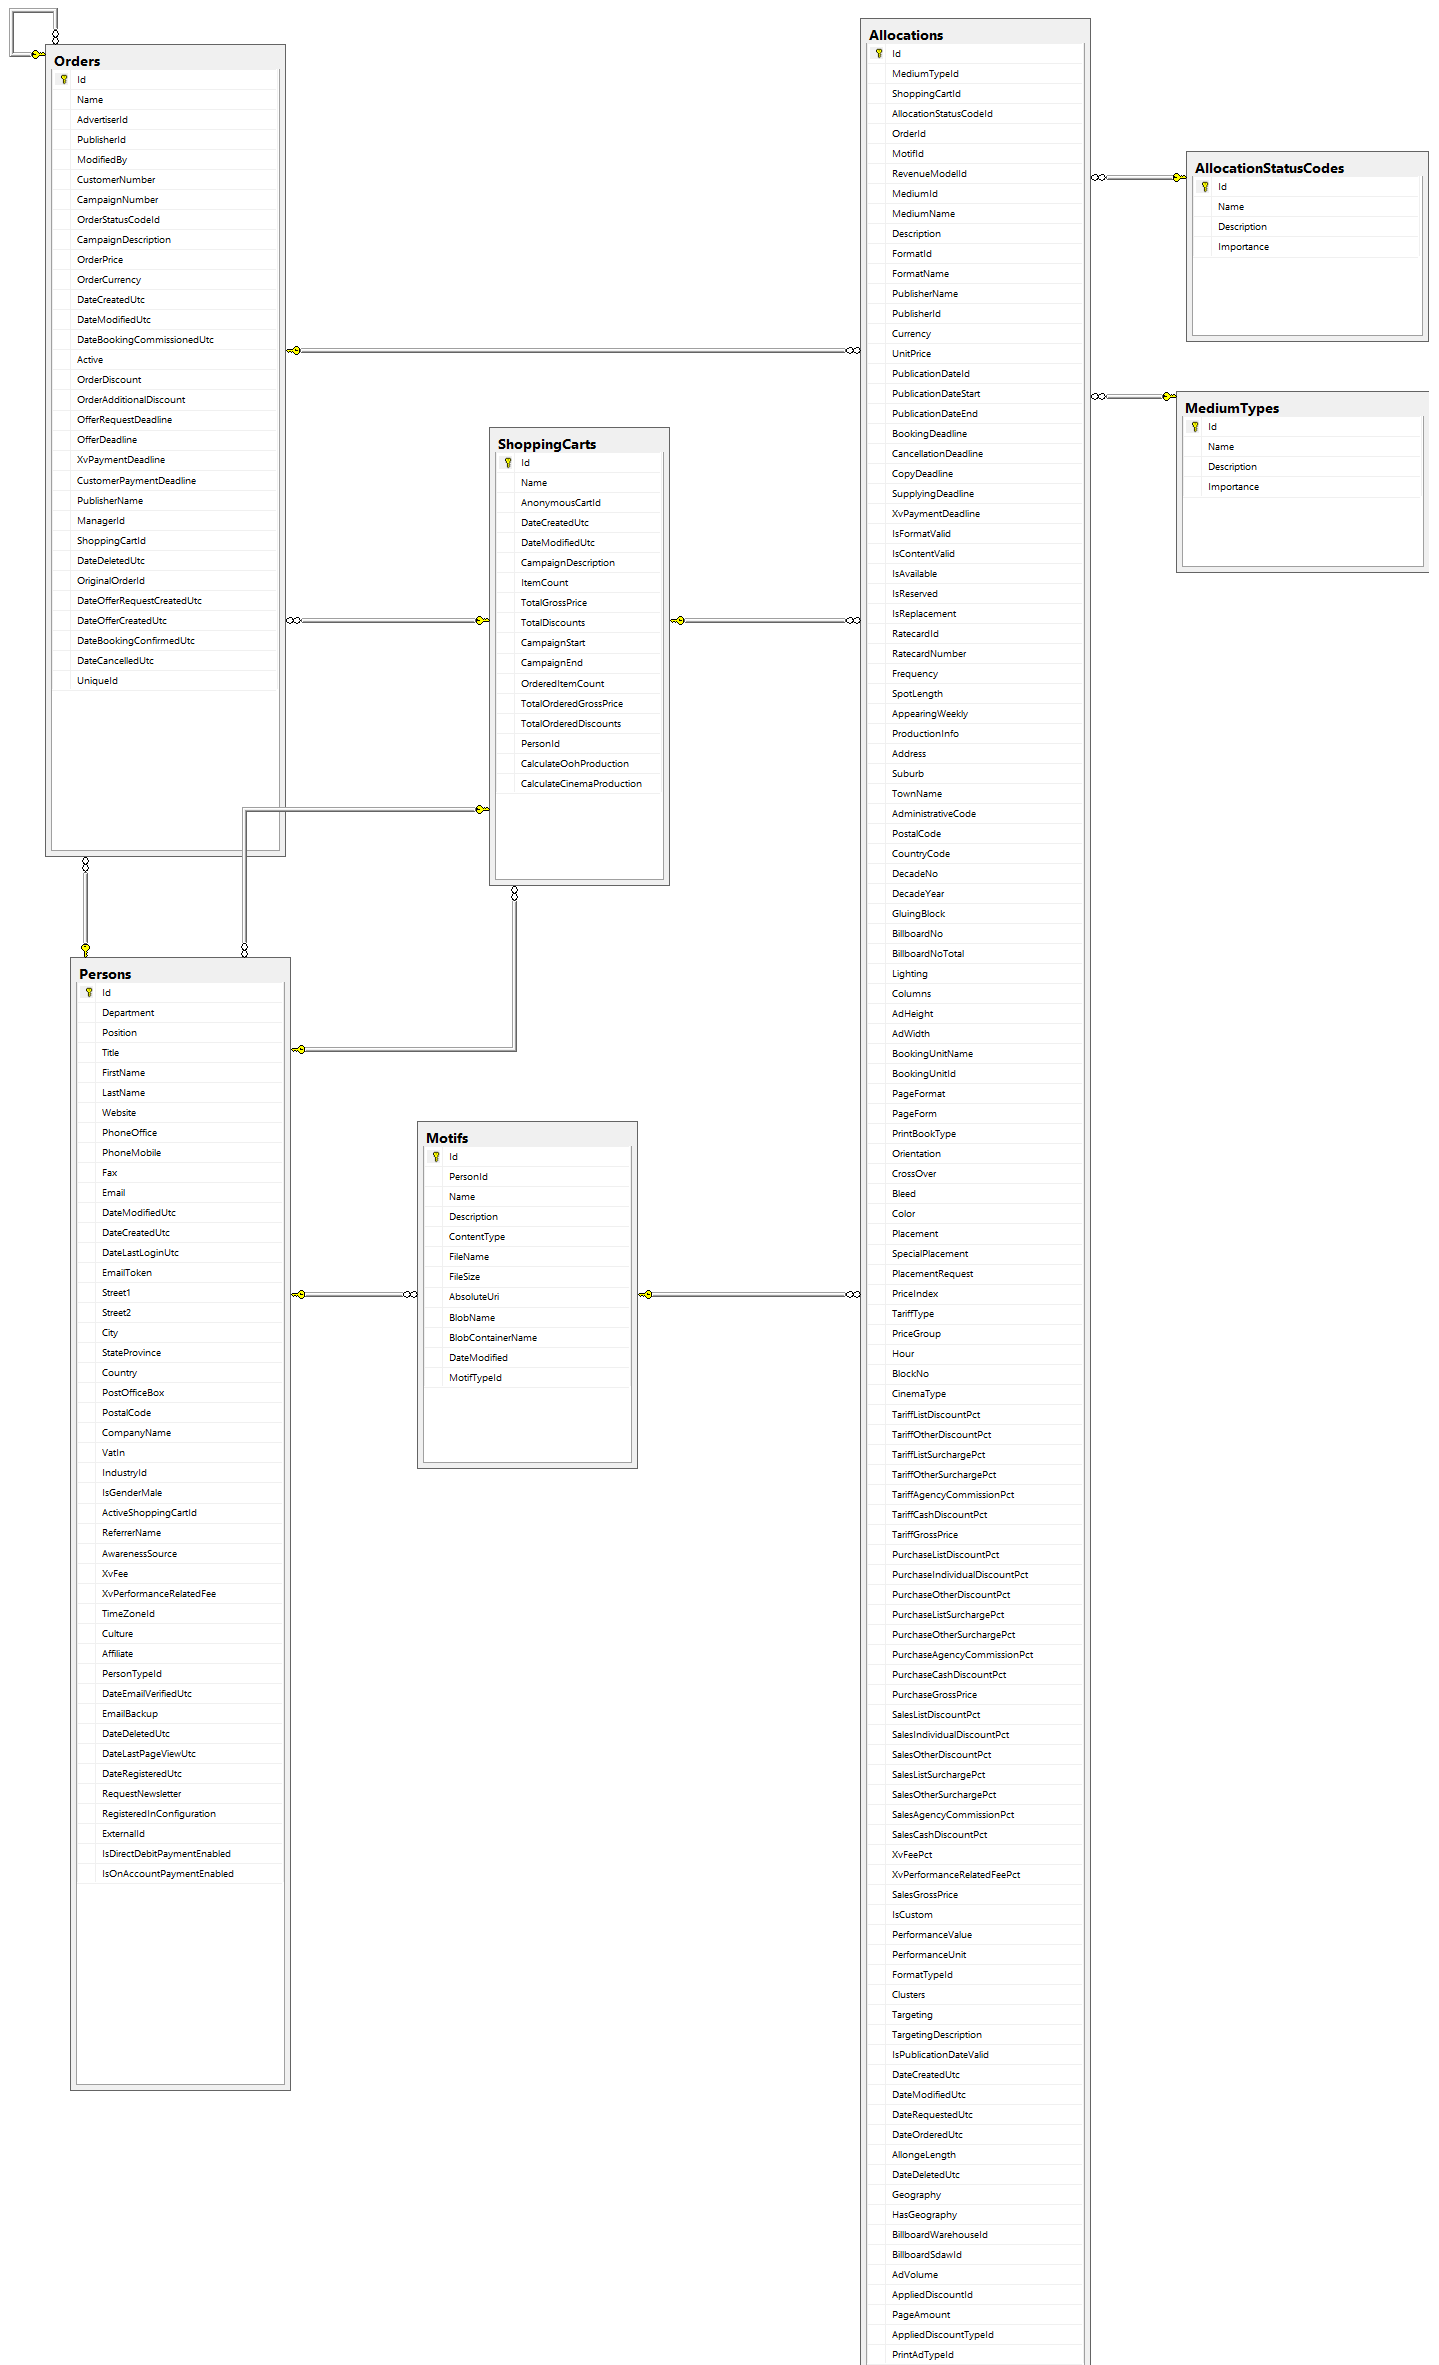
\includegraphics[width=\textwidth]{core_erd}
\caption{XV Marketplace ERD}
\label{fig:xv_erd}
\end{figure}

\begin{figure}
\centering
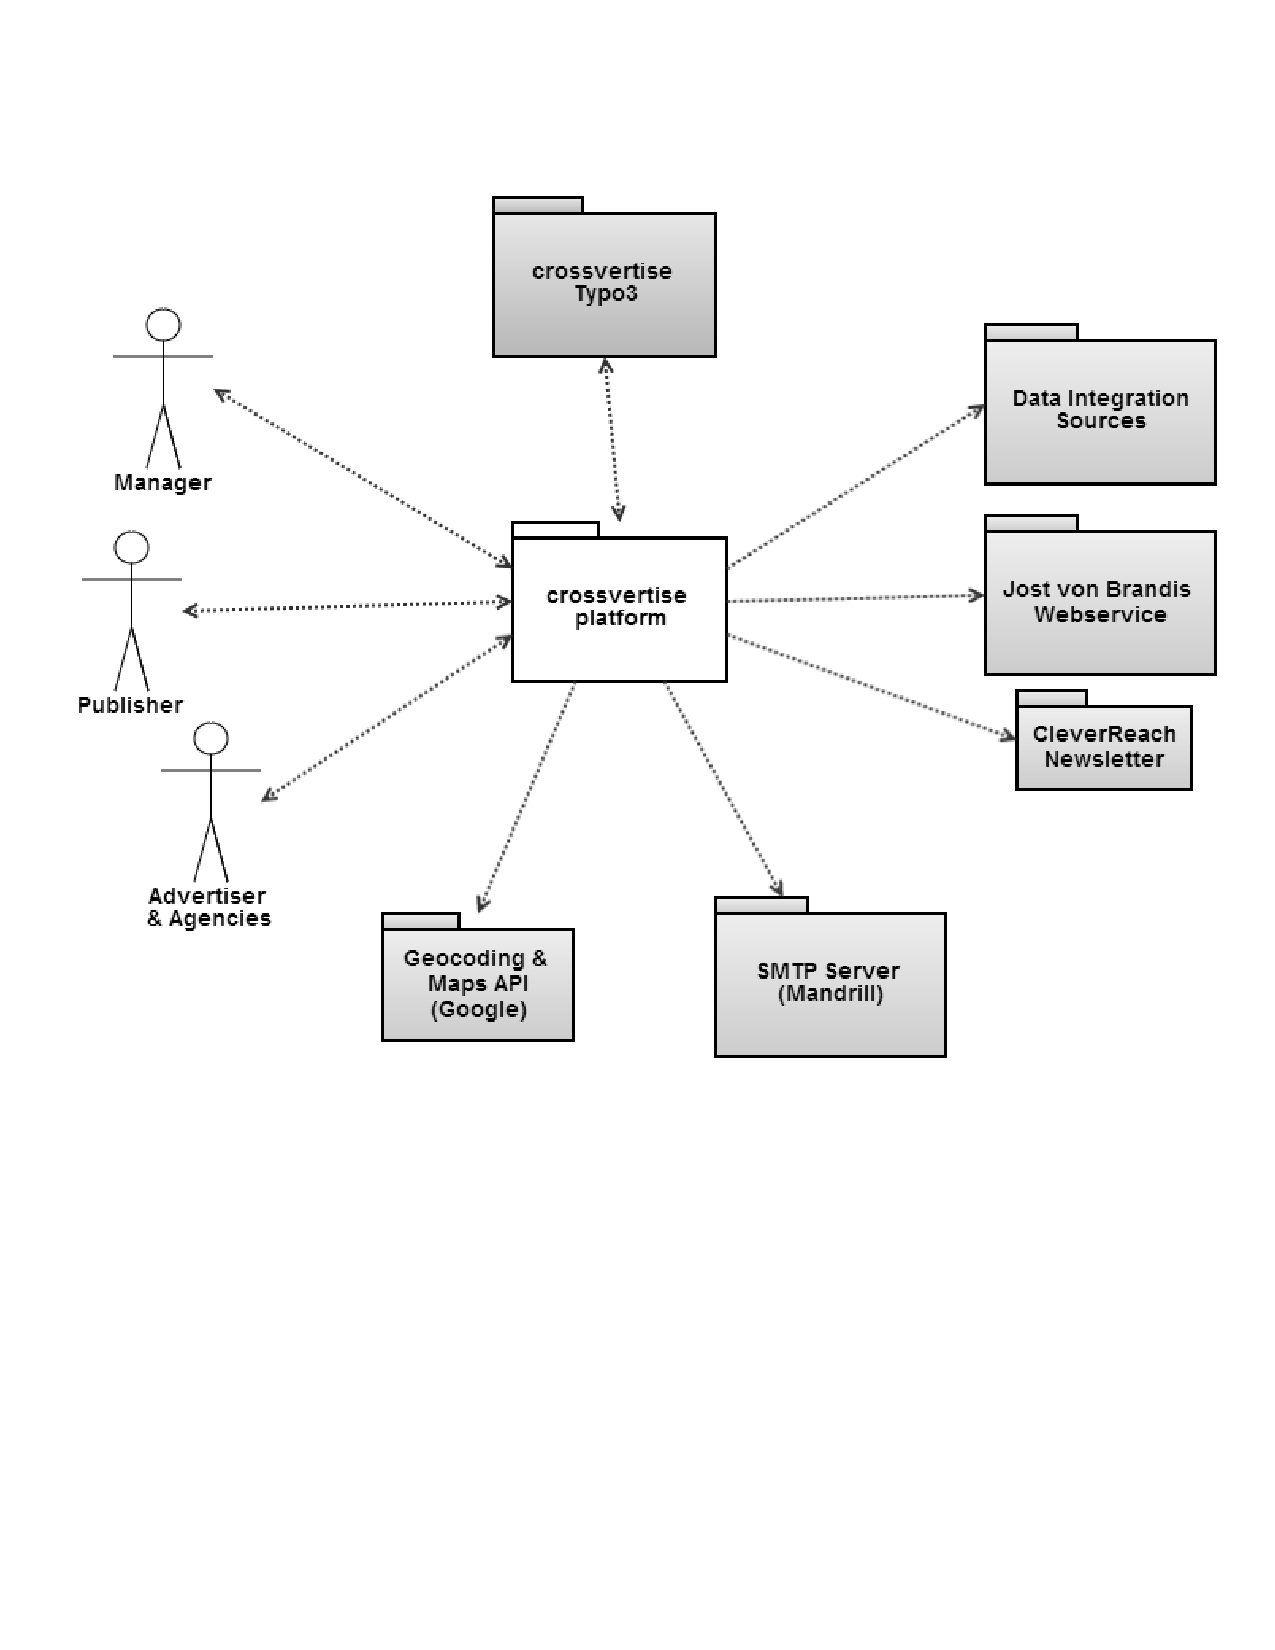
\includegraphics[width=\textwidth]{cross_use_case}
\caption{XV Package Diagram}
\label{fig:cross_use_case}
\end{figure}

\begin{figure}
\centering
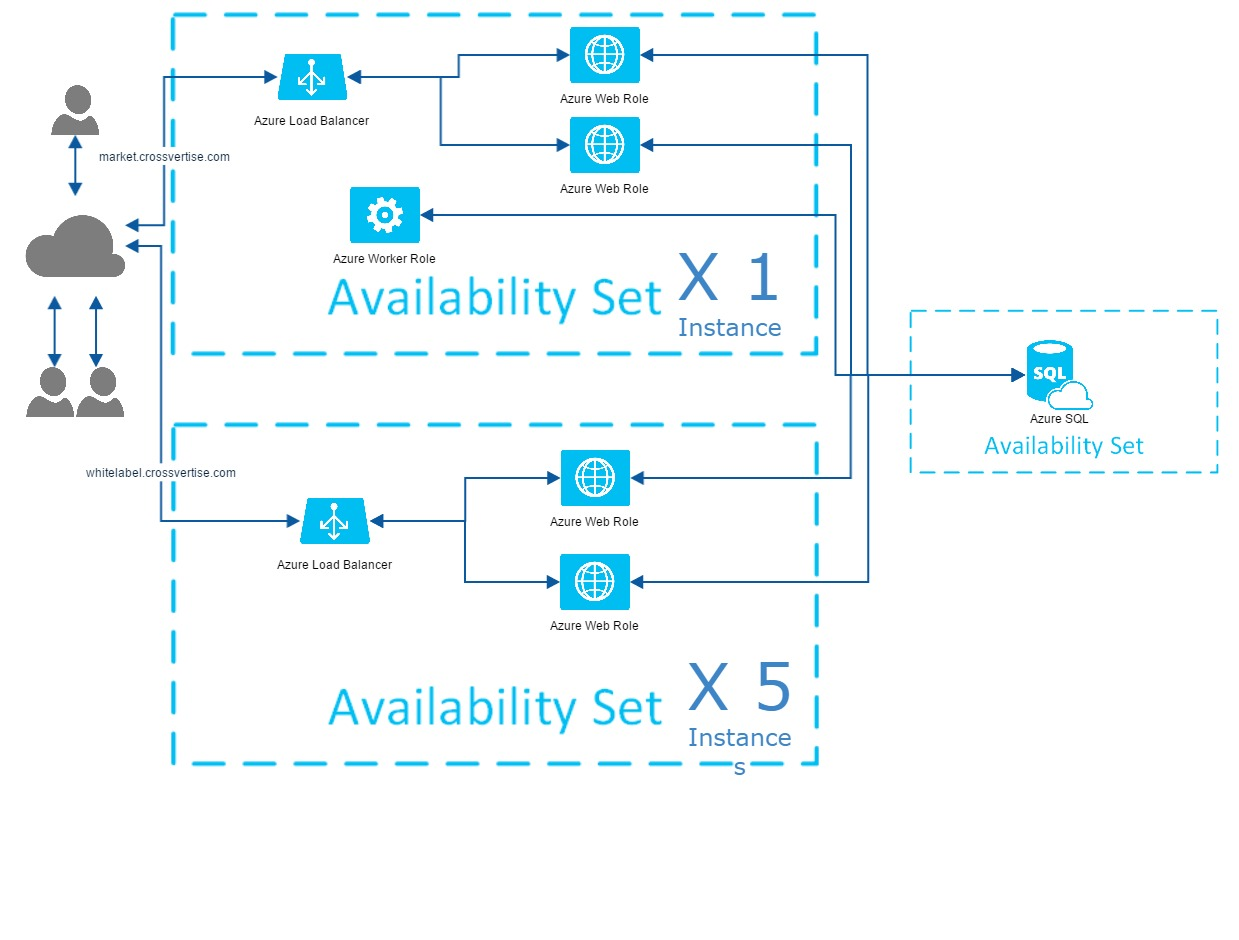
\includegraphics[width=\textwidth]{xv_azure_arc}
\caption{XV Conceptual Architecture Blueprint}
\label{fig:xv_azure_arc}
\end{figure}

\begin{figure}
\centering
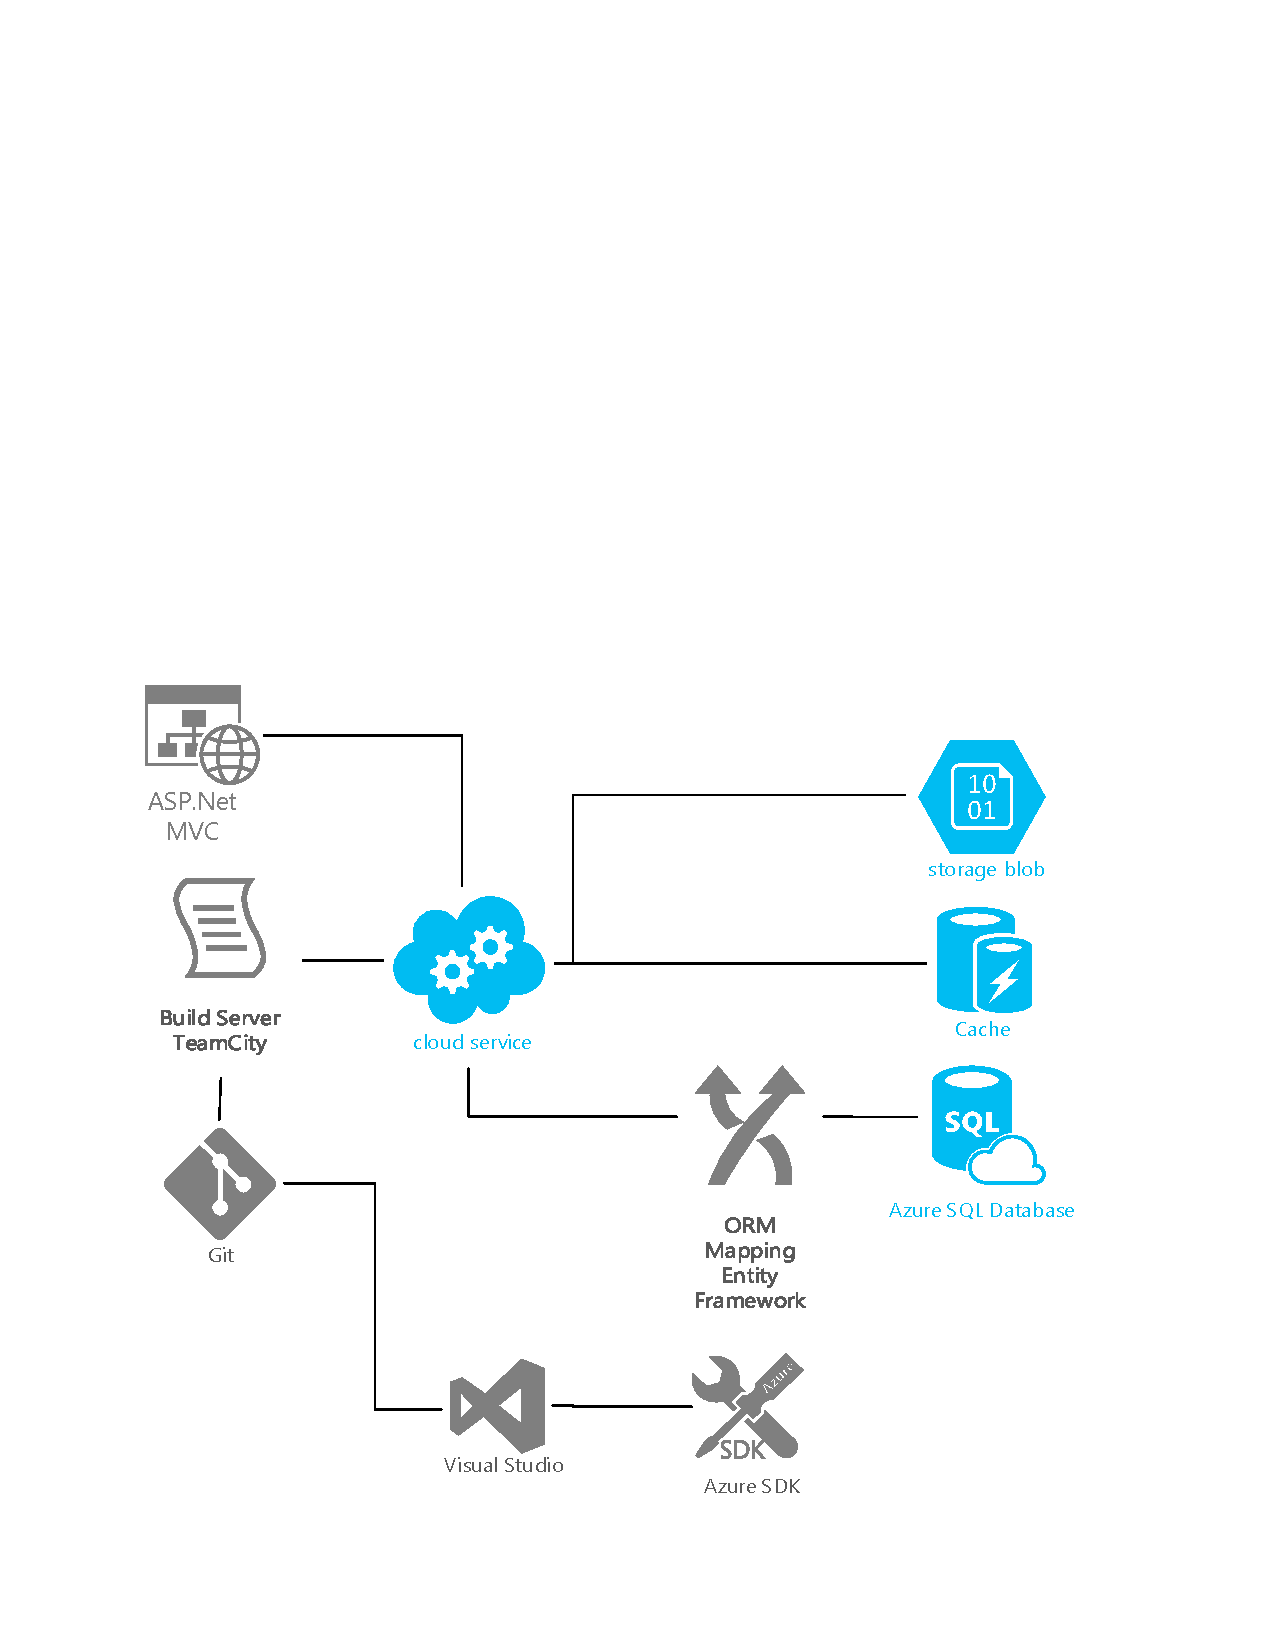
\includegraphics[width=\textwidth]{tech_breakdown}
\caption{XV Technology Breakdown}
\label{fig:tech_breakdown}
\end{figure}

\begin{figure}
\centering
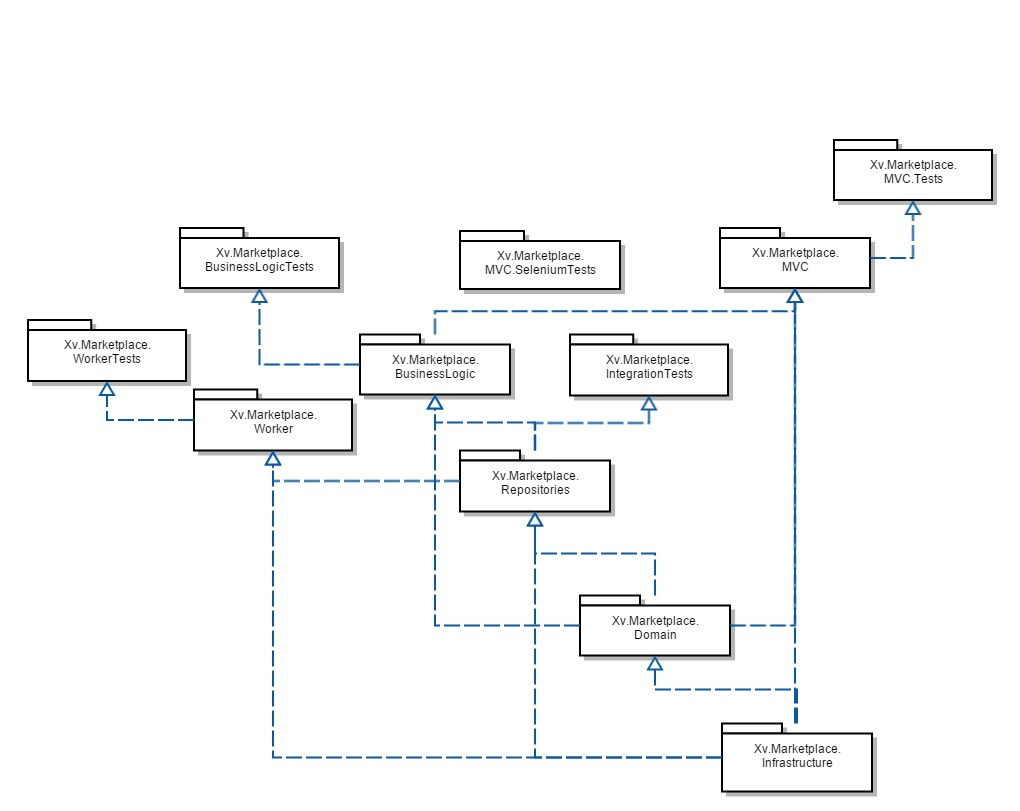
\includegraphics[width=\textwidth]{xv_proj_arc}
\caption{XV Package Diagram}
\label{fig:xv_proj_arc}
\end{figure}
%\chapter{List of Abbreviations}



\begin{table}[h]
\centering
\begin{tabularx}{\textwidth}{l X l}
ACID        & Atomicity, Consistency, Isolation and Durability  &  \\
AD          & Architecture description &  \\
ADL         & Architecture Description Languages &  \\
AES         & Azure Elastic Scaling                  &  \\
ASP         & Application service provider &  \\
BASE        & Basically Available, Soft State and Eventually Consistent & \\
BI          & Business identity                                                                                     &  \\
CI          & Corporate identity                                                                                    &  \\
CQRS        & Command Query Responsibility Segregation   &  \\
CRUD        & Create, Read, Update and Delete           &  \\
CSS         & Cascading Style Sheets                                                                                &  \\
DDD         & Domain Driven Design                                                                                  &  \\
DI          & Dependency Injection                                                                                  &  \\
DNS         & Domain Name System                                                                                    &  \\
IaaS        & Infrastructure as a Service   &  \\
IIS         & Internet Information Services &  \\
IoC         & Inversion of Control                                                                                  &  \\
IT          & Information Technology                                                                                &  \\
MAF         & Managed Addin Framework                                                                               &  \\
MEF         & Managed Extensibility Framework &  \\
MSQ         & Multi-Shard Queries                                                                                   &  \\
MVC         & Model, View Controller                                                                                &  \\
OCP         & Open/Close principle                                                                                  &  \\
OMG         & Object Management Group                                                                               &  \\
ORM         & Object Relational  &  \\
PaaS        & Platform as a Service                                                                                 &  \\
POCO        & Plain Old CLR Object                                                                                  &  \\
QCW         & Queue Centric Workflow                                                                                &  \\
SaaS        & Software as a Service                                                                                 &  \\
SLA         & Service Level Agreement                                                                               &  \\
SMB         & Server Message Block                                                                                  &  \\
SP          & Service providers                                                                                     &  \\
SS          & Service Science                                                                                       &  \\
UI          & User Interface                                                                                        &  \\
UML         & Unified Modelling Language  &  \\
VHD         & Virtual Hard Drive                                                                                    &  \\
VPN         & Virtual Private Network                                                                               & \\
\end{tabularx}
\end{table}
%\chapter{Windows Azure as Reference Technology}

\end{document}

